\section{METHODOLOGY}

The first step was to define mathematical models of the prototype vehicle DT1 and the track. 
A formulation was then proposed for the optimal control problem (OCP) to find the optimal driving strategy and gear ratio. 
Accordingly, this proposed OPC was solved utilizing MATLAB and the FALCON.m library.

\subsection{Modeling of vehicle dynamics}

A simple model of the vehicle's dynamics was used. 
Only the longitudinal dynamics was modeled. Aerodynamic drag did not consider wind effect. 
Tire rolling resistance was independent of temperature, pressure, or speed. 
Bearing friction was zero. The battery and power converter were treated as ideal. 
The dynamics of the inductor in the motor were disregarded. 
A white-box model was derived by using the fundamental principles that describe the system's behaviour. 
The following equation that describes the longitudinal dynamics was derived from the application of Newton’s second law in the vehicle, as represented in Fig.~\ref{fig:diag_forcas_veiculo}. 

\begin{equation} \label{eq:modelo_1}
	\begin{split}
		\left( m_v + m_p + m_r \right) \ddot x(t) = F_t - (F_a + F_g + F_r) \enspace,\\ 
		m_r = \frac{N_r \cdot J_r + J_m\cdot \varphi^2 }{r_r^2} \enspace,\\ 
		F_{t} =  K_t \cdot i(t) \cdot \eta \cdot \frac{\varphi}{r_r} \enspace,\\
        F_{a} = \frac{\rho \cdot a_f \cdot c_d \cdot {\dot x(t)}^2}{2} \enspace,\\
        F_{g} = (m_v + m_p) \cdot g \cdot \sin(\theta(x)) \enspace,\\
        F_{r}  = c_{r} \cdot (m_v + m_p) \cdot g \cdot \cos(\theta(x)) \enspace,
	\end{split}
\end{equation}


\noindent where $m_v$ is the mass of the vehicle, $m_p$ is the mass of the pilot, $m_r$ is mass equivalent to the moment of inertia of the rotating parts 
(i.e., wheels and engine axle), $x$ is the position, $\varphi$ is the gear ratio, $F_{t}$ is the propulsive force, $i$ is the electric current in the motor, $F_{a}$ is the aerodynamic drag, $F_g$ is the component 
of the weight that is the direction of speed, $F_{r}$ is the rolling resistance of tires on the track, and $\theta$ is the slope of the track. The model constants are shown in Tab. \ref{tab:constantes}.
The experimental validation of this model has not been performed.

\begin{figure}[h]
	\centering
	\begin{normalsize}
		\import{2_Desenvolvimento/Figuras/}{diagrama_forcas_veiculo.pdf_tex}
	\end{normalsize}
	\caption{Diagram of forces of a moving vehicle}
	\label{fig:diag_forcas_veiculo}
\end{figure}

\begin{table}[!h]
	\centering
    \caption{Constants used in the vehicle model}
	\label{tab:constantes}
	% \rowcolors{1}{}{lightgray}
	\begin{tabular}{llll}
		\toprule
		\textbf{Constant} & \textbf{Symbol} & \textbf{Value} & \textbf{Unit}\\
		\midrule
		Vehicle mass                    & $m_v$  & 36               & \si{kg}                \\
        Pilot mass		                & $m_p$  & 50               & \si{kg}                \\  
        Number of wheels                & $N_r$  & 3                & -                      \\
        Moment of inertia of the wheel  & $J_r$  & 0.015            & \si{kg.m^{2}}          \\
        Moment of inertia of the motor  & $J_m$  & \num{0.0625d-3}  & \si{kg.m^{2}}          \\
        Wheel radius                    & $r_r$  & 0.254            & \si{m}                 \\
        Torque constant                 & $K_t$  & 0.119            & \si{N.m / A}           \\
        Transmission efficiency         & $\eta$ & 0.95             & -                      \\
        Air density                     & $\rho$ & 1.22             & \si{kg / m^{3}}        \\
        Frontal area of the vehicle     & $a_f$  & 0.26             & \si{m^{2}}             \\
        Aerodynamic drag coefficient    & $c_d$  & 0.164            & -                      \\
        Gravity acceleration            & $g$    & 9.81             & \si{m / s^{2}}         \\
        Rolling resistance coefficient  & $c_r$  & 0.0024           & -                      \\
		\bottomrule
	\end{tabular}
\end{table}

\subsection{Track modeling}

In 2018 and 2019, SEM Americas was held at the Sonoma Raceway. 
It is expected that the track will remain the same for the next editions of the competition. 
\citet{site:dados_sonoma} made available GPS data collected on the Sonoma Raceway track in 2018. 
This data were used for track modeling. The layout of one lap in Sonoma Raceway is shown in Fig.~\ref{fig:pista}, peaks of elevations are indicated with a triangle, valleys with a square. 

The track’s relative altitude $h$ was approximated by a sum of sines with 8 terms
\footnote{The fit was implemented in MATLAB using the command \lstinline[style=Matlab-editor]{fit(x, h, 'sin8')}}.  
The approximation with trigonometric functions was chosen because of the periodicity of these functions. 
In this way, it would be possible to represent all track laps in a continuous function. 
Using continuous functions instead of interpolating values in tables reduces the computational cost.
The slope model $\theta$ was obtained by deriving the altitude model with respect to $x$:
\[ \theta(x) = arctg\left( \frac{\mathrm{d}h(x)}{\mathrm{d}x}  \right)  \]
\begin{equation}
	\label{eq:modeloTheta}
	\theta(x) = \operatorname{arc\,tan} \left( \sum_{n = 1}^{8} a_n \cdot \cos(b_n \cdot x + c_n) \right)
	\enspace,
\end{equation}

\noindent where the coefficients $a_n$, $b_n$ and $c_n$ are presented in Tab.~\ref{tab:coeficientes}. The fitted curve and the data are displays in Fig.~\ref{fig:altitude_pista}


\begin{figure}[!h]
    \centering
    \begin{minipage}{.5\textwidth}
        \centering
        % This file was created by matlab2tikz.
%
%The latest updates can be retrieved from
%  http://www.mathworks.com/matlabcentral/fileexchange/22022-matlab2tikz-matlab2tikz
%where you can also make suggestions and rate matlab2tikz.
%
%
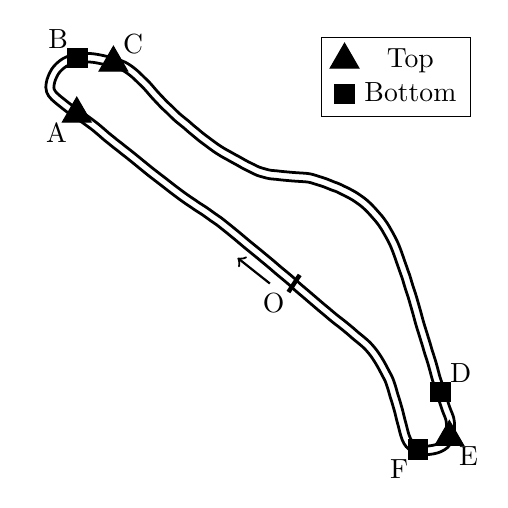
\begin{tikzpicture}

\begin{axis}[%
% width=4.521in,
% height=3.566in,
width=2.2605in,
height=2.26in,
at={(0.758in,2.6in)},
scale only axis,
xmin=-330,
xmax=230,
ymin=-230,
ymax=300,
axis background/.style={fill=white},
axis line style={draw=none},
xtick=\empty, ytick=\empty
]
\addplot [color=black, line width=1pt, forget plot]
  table[row sep=crcr]{%
-4.73238656650697	-2.60902398256989\\
-7.89283938896916	-0.0585958241745614\\
-10.9651059143732	2.41161254599027\\
-14.0610317515681	4.86135937341073\\
-17.1987793236763	7.30667812541416\\
-20.3596019737996	9.77154506542119\\
-23.5075643844916	12.2515498453164\\
-26.7424077140927	14.9230253918275\\
-29.6878625140287	17.346074118677\\
-32.8977313881561	19.8969894998738\\
-35.9745554100071	22.3478798814084\\
-39.0461693558466	24.7406500248347\\
-42.2515954117174	27.2330340332547\\
-45.4676307488345	29.8064148818835\\
-48.4484940144044	32.1283435347169\\
-51.6821193850276	34.5763045056348\\
-54.8349436668391	37.01752287053\\
-57.9654198702129	39.433279596167\\
-61.1878463670267	41.9099306938153\\
-64.4276584524961	44.4815039464233\\
-67.4398138638897	46.8843555357432\\
-70.6671230873407	49.4463357464304\\
-73.7881950060064	51.9583793090802\\
-76.7904582354019	54.2871147715348\\
-80.0525081705761	56.7864468591972\\
-83.2382781086666	59.2814028819272\\
-86.2849115378886	61.5828191781599\\
-89.5663335915205	64.0372807509451\\
-92.7080819519192	66.4455088746133\\
-95.8137128415046	68.7452291628735\\
-98.794079361641	70.7025356920541\\
-102.379021650371	72.9768418706848\\
-105.754283493198	75.2920721976301\\
-108.95813702547	77.482811020808\\
-112.314743509257	79.7415842892376\\
-115.466108795471	81.7643537352265\\
-118.868482986499	83.7975663583247\\
-122.438209019836	85.9661521713886\\
-125.911429360208	88.2035589101987\\
-129.169862746059	90.326210871217\\
-132.498498036343	92.4272441190572\\
-135.998437218732	94.6732913901229\\
-139.353263710683	96.9181131991431\\
-142.714410097924	99.2269583696576\\
-146.033700416929	101.560079799244\\
-149.244503495514	103.826042386363\\
-152.531271526526	106.162001166731\\
-155.857673929233	108.61689189914\\
-158.978573374941	110.927502759444\\
-162.276044609052	113.339748283371\\
-165.491460242591	115.72892687825\\
-168.609229667658	117.99344037314\\
-171.967189227966	120.421178494994\\
-175.154440338945	122.742179308557\\
-178.438124015609	125.145093285276\\
-181.592801342342	127.472809887493\\
-184.949647483525	130.054437174848\\
-187.953627242841	132.389289757053\\
-191.212392214781	134.874994788373\\
-194.34617585508	137.310741355512\\
-197.548811376719	139.812407239064\\
-200.659020878355	142.200411618347\\
-203.91876998839	144.704834413093\\
-206.967783854515	147.032942404613\\
-210.152839329549	149.37088081804\\
-213.415490606613	151.786746064536\\
-216.636084739556	154.206175669978\\
-219.830169868052	156.615865504569\\
-222.865521265795	158.815924537745\\
-226.365938508548	161.425384138848\\
-229.452056274277	163.848439185807\\
-232.535704674991	166.15635995038\\
-235.943147592981	168.78974431836\\
-239.041720345914	171.352754549496\\
-242.090324077265	173.884133533313\\
-245.125475379374	176.323259890661\\
-248.348767077197	178.905632575635\\
-251.176057583704	181.033509301001\\
-254.549923545949	183.419655085213\\
-257.672694086407	185.603530494622\\
-261.056313361613	187.92732419315\\
-264.171221566164	189.987104768033\\
-267.449836678907	191.957123116321\\
-271.084938468976	194.21321151303\\
-274.373797188289	196.355810147903\\
-277.870937190664	198.707262448665\\
-281.171331525877	201.051753450223\\
-284.422066489836	203.361079051739\\
-287.836731937087	205.883425044657\\
-290.951711229744	208.256564640249\\
-294.150421101231	210.657530027144\\
-297.500608389416	213.368105673614\\
-300.483451093876	215.93010902325\\
-304.011158856039	219.827483899135\\
-306.422590444573	224.188268981344\\
-307.550609136123	230.199868599406\\
-307.044071915564	234.902663888923\\
-306.033149891746	239.253168389228\\
-304.318423989251	243.764827698065\\
-302.53963905227	247.429953482638\\
-300.177916028709	251.450128903403\\
-297.209053570142	255.155769515505\\
-293.890050419873	258.342271663906\\
-290.61599050606	260.981195813918\\
-286.649107154644	263.586293234018\\
-282.434954585847	265.559954923848\\
-278.383497135923	267.000712245562\\
-274.35315674267	268.240302141386\\
-269.774555216509	269.222801703332\\
-265.535224713127	269.698651458296\\
-261.273088506036	269.937702071831\\
-257.018626097863	269.918821878033\\
-252.892687411758	269.719565788121\\
-248.670600528564	269.363538578467\\
-244.391017404692	268.7840999477\\
-240.394369886023	268.080199794235\\
-236.43427259268	267.320916798851\\
-232.292101076934	266.413831810356\\
-228.109329677082	265.252333707912\\
-224.392744184788	264.119267284812\\
-220.67822371318	263.088755629493\\
-216.846055860323	262.099575222759\\
-212.771836761231	260.959863150358\\
-208.149494171033	259.033175752892\\
-204.548205520746	256.985770940224\\
-200.898684172864	254.661682817844\\
-197.476365038245	252.217471816168\\
-194.14229121012	249.597718336752\\
-190.94171197296	246.808817036745\\
-187.939216299443	244.041065475051\\
-184.996451278915	241.314713853432\\
-182.073412621385	238.625931845484\\
-179.027487960424	235.7361081165\\
-176.086214693457	232.672159093702\\
-173.383835923788	229.647600393508\\
-170.795770802807	226.794426397805\\
-168.110015552462	223.962443812261\\
-165.359753949486	221.164694020225\\
-162.488754879711	218.295930209478\\
-159.700291547079	215.517001796865\\
-156.928116467472	212.816351340858\\
-154.221922918165	210.407582060605\\
-151.027045043783	207.644137841897\\
-147.968602224376	204.796441253474\\
-145.12304088803	202.117493014745\\
-142.246686477318	199.500539763656\\
-139.468424243858	197.231589771094\\
-136.177648404639	194.726690851998\\
-133.106105969561	192.380905042624\\
-129.876783363463	189.905519397641\\
-126.529532924421	187.07118323573\\
-123.822071535229	184.824429238928\\
-120.584579799111	182.357273249831\\
-117.366668723585	179.820439310081\\
-114.263797116311	177.352676226061\\
-111.188489459749	175.014234741249\\
-108.064685574186	172.78485782333\\
-104.77016658539	170.486039657237\\
-101.491318063615	168.16861077756\\
-98.2563060521595	165.90076637304\\
-94.971519031186	163.642812361349\\
-91.8495227996287	161.636034312079\\
-88.4136463802549	159.545742056473\\
-85.1891176228038	157.68636611086\\
-81.801122895254	155.925428725535\\
-78.0830904567754	153.983835328028\\
-74.6234921721756	152.131923228786\\
-71.1213077993493	150.318363624992\\
-67.5944673386654	148.517936545315\\
-63.8777972343759	146.533575244518\\
-60.4761311486314	144.684104805746\\
-57.0342212475474	142.934462647757\\
-53.5874771366474	141.34005049262\\
-49.7252882864552	139.539659360337\\
-46.18956117614	137.817267656845\\
-42.9083776220702	136.407481725131\\
-39.666369208144	135.385404389109\\
-35.7453336613009	134.372876271339\\
-31.901453071837	133.351848488906\\
-28.6485001228393	132.730369911948\\
-24.9563585983061	132.405640785863\\
-20.7242757138278	132.051977353971\\
-16.6953550148376	131.593077127364\\
-12.8991457162293	131.219233657856\\
-8.87526621671924	130.885361955645\\
-4.87172738754626	130.528998365233\\
-1.01567876995557	130.209806675548\\
2.90126173990634	129.942119451001\\
6.89880130572476	129.705856152961\\
10.9278568816854	129.473851258788\\
14.994738323859	129.196413277665\\
19.3518302682471	128.686143651904\\
23.818567951474	127.704521747567\\
27.7880472537492	126.515441204451\\
31.504163608366	125.389738493466\\
35.3555240690361	124.29768444187\\
39.5056509963823	122.983670355183\\
43.3650238273162	121.544144800964\\
47.0700966544626	120.127377806321\\
50.8892938918558	118.638349413523\\
53.9525037532504	117.664272479604\\
59.0391732705182	115.596254130914\\
61.8956744057682	114.173929277403\\
65.8300476805389	112.452863619829\\
69.5762950783508	110.625961623432\\
73.1359711012941	108.831559150249\\
76.9140402187221	106.791664478392\\
80.5454605431881	104.554735894375\\
83.9250520556913	102.30079358416\\
87.2583720920615	100.017155741827\\
90.7711485830888	97.3532443307433\\
94.0154043357183	94.4972123899162\\
96.9592126426863	91.737649189798\\
99.9666541670764	88.7753955352927\\
102.78460019488	85.7966589705356\\
105.502773758839	82.8788293454264\\
108.292863343777	79.8550249997061\\
111.08113373033	76.5546602700026\\
113.583712260695	73.2405295971062\\
115.93617198821	69.9388347940886\\
118.312470235191	66.2564430394441\\
120.368962055431	62.7868975142443\\
122.423553808867	59.3682978521217\\
124.54756176914	55.6417910360586\\
126.406796611125	52.223139970718\\
128.382509454075	48.2849904214194\\
130.02780146007	44.6049482003815\\
131.654595601188	40.7238373953991\\
133.118239721736	36.9577388882666\\
134.537766572453	33.1594777709772\\
135.918635100333	29.3530573886741\\
137.290699840753	25.6315987868825\\
138.701515317503	21.9069017833792\\
140.104213860124	18.0996011350233\\
141.431994159074	14.4691824933215\\
142.840215052553	10.8375461486692\\
144.311341567293	6.53486722204021\\
145.435927100324	2.82447785162349\\
146.651016366046	-0.931869388917319\\
147.887053313733	-4.71847386169747\\
149.134305296758	-8.26100586570684\\
150.539398785027	-12.199944710644\\
151.817846431873	-16.1205701772408\\
153.005615767889	-20.1058079091772\\
154.093724287177	-23.7166406953759\\
155.317701105057	-27.6730980176675\\
156.452648844799	-31.4965769155037\\
157.590575253269	-35.4120479444184\\
158.677865670897	-39.2811102162789\\
159.762597054294	-43.0300719016368\\
160.9197553921	-46.8068664329385\\
162.127846729139	-50.6022320531358\\
163.3554955285	-54.2477624490664\\
164.667513467389	-58.1855368777564\\
165.887136382035	-62.0133946903123\\
167.116755242715	-65.7430714841902\\
168.398499582795	-69.5665847420466\\
169.634974305547	-73.6223361989428\\
170.725854190368	-77.2392665754502\\
171.948947466435	-80.9050444433333\\
173.244768503186	-84.673565157248\\
174.5603670886	-88.5321103594271\\
175.816382818875	-92.5037613231765\\
176.948574008273	-96.3316268468371\\
178.07516578893	-100.230550783254\\
179.150869513685	-104.13758219127\\
180.212023801598	-107.915855804586\\
181.353500815093	-111.471759958763\\
182.669133238087	-115.181617800726\\
183.995557652315	-119.244605405915\\
185.145004777531	-123.03501174266\\
186.337025820032	-126.958887548448\\
187.481187053129	-130.22452759345\\
188.990771050589	-134.16147381027\\
190.35106221487	-137.966547382178\\
191.672079392948	-141.757415066363\\
192.975110880458	-145.381383332428\\
194.384442548563	-148.88835406649\\
195.953144042691	-152.425855078302\\
197.591343632798	-156.89872843854\\
198.497410353015	-161.634988090118\\
198.798391394146	-166.044972521666\\
198.754637665533	-170.414136729587\\
198.437602771983	-174.683800615099\\
197.65957013364	-179.249426081656\\
196.081091312305	-183.902598514296\\
193.868209146235	-188.029833335734\\
190.310042910658	-192.135892761611\\
186.284260385131	-195.011667173174\\
182.206223148917	-197.070739705986\\
177.886441912141	-198.612319859321\\
173.414206177984	-199.620280751486\\
169.297882493636	-200.241667246531\\
164.91043559313	-200.641789597692\\
160.542793900447	-200.69583938203\\
155.832824254913	-200.227226235001\\
151.35902848966	-199.160029930101\\
146.856776602027	-197.364153495651\\
142.78212102211	-194.920390815717\\
138.952785976461	-191.478727591967\\
136.105861421973	-187.66260176603\\
133.873510626759	-183.198891756612\\
132.46456823375	-179.316023477929\\
131.182967107325	-175.149088085413\\
130.146687145805	-171.14882425582\\
129.16316582771	-167.458161146447\\
128.073632013942	-163.668770371653\\
126.969372068832	-159.708197232558\\
125.938647602133	-155.716481577071\\
124.97155615596	-151.885394069675\\
123.941237197623	-148.316143263819\\
122.730626161416	-144.415299319114\\
121.583689687623	-140.6056259504\\
120.40572074922	-137.042208928714\\
119.067892370229	-133.110999571277\\
117.87211322586	-129.158400583473\\
116.776719402138	-125.427440790027\\
115.601762315197	-121.789985537147\\
114.292931524982	-118.067331645023\\
112.938608465798	-114.737755844022\\
111.328379020242	-111.594457037056\\
109.328711471661	-108.056742062542\\
107.367001480716	-104.552952327915\\
105.400977002647	-100.993831937512\\
103.514026263549	-97.7126798218527\\
101.445932972948	-94.3342559801604\\
99.3927737397856	-91.1862693406631\\
97.141753124057	-87.9255507744207\\
94.9680224668095	-84.9920541008122\\
92.5590143690601	-82.0877697979861\\
89.9782073771724	-79.1687202617677\\
87.4324774086506	-76.5280250617184\\
84.7773262422367	-74.1688856482907\\
81.6679828885499	-71.6276936783907\\
78.6653074147493	-69.2475702873308\\
75.5182532291431	-66.8851409901199\\
72.1590650075697	-64.2270229837538\\
69.1178041928673	-61.6766308196025\\
66.0855540622897	-59.1843113010962\\
63.0413873534316	-56.7847403209303\\
59.8419589466482	-54.3112949811606\\
56.711932608885	-51.893701352171\\
53.6416518710089	-49.6371650660026\\
50.3649777999799	-47.3061615955092\\
46.9800337570735	-44.7492215429701\\
43.8611248336124	-42.3050806152286\\
40.6047665167058	-39.7099104953934\\
37.5449492214464	-37.2011309316973\\
34.5833412278778	-34.902004727165\\
30.406442744474	-31.6441910615212\\
27.195878225692	-29.0403898057287\\
24.6776467349898	-26.9907014491863\\
21.668728553742	-24.5469747312195\\
18.8175080510238	-22.2505008420462\\
15.7028529013626	-19.7278447637192\\
12.6046209458534	-17.1919483131002\\
9.52120702031128	-14.7126582600479\\
6.36063004520681	-12.2130128305592\\
3.18109748715986	-9.63899967540168\\
0.114082434129711	-7.13623944708169\\
-4.73238656650697	-2.60902398256989\\
};
\addplot [color=black, line width=1pt, forget plot]
  table[row sep=crcr]{%
1.53880524038682	5.18020918386878\\
-1.60376882250141	7.71620908720354\\
-4.72234695245479	10.2236520071929\\
-7.8926318312805	12.7322451192081\\
-11.0736749257357	15.2113031079373\\
-14.1860667646708	17.6384035884689\\
-17.3043039520425	20.094990417362\\
-20.2129611828268	22.4970816363599\\
-23.5091587278328	25.2088738441213\\
-26.632083520547	27.6906828989706\\
-29.7793771155531	30.1977057329751\\
-32.9511580152136	32.6685019884852\\
-36.0715036092345	35.0947428368726\\
-39.1514382023042	37.5592022332273\\
-42.4770584139974	40.1496873666562\\
-45.5814635912246	42.4998137588343\\
-48.6912963227732	44.9077444968058\\
-51.8900789988428	47.3762156588997\\
-55.0757821143021	49.8246429798409\\
-58.103872865773	52.2280990599653\\
-61.2912584569447	54.7707530915178\\
-64.3826750928959	57.2248776024031\\
-67.5330001083875	59.7604647221479\\
-70.7898622718837	62.2866677642095\\
-73.892100298009	64.6635894149477\\
-77.0671079965627	67.1501168459417\\
-80.4040359061352	69.6707918415563\\
-83.4676113358817	71.9622783439148\\
-86.6393056858445	74.3934617325716\\
-89.9820779031658	76.8687772759794\\
-93.6604487492843	79.2842509481014\\
-96.8043529482077	81.2788337317453\\
-100.015956662378	83.4817977841616\\
-103.407729294034	85.8010424443025\\
-106.699329345061	88.0160706034776\\
-110.282054772334	90.3157035634813\\
-113.792553387588	92.4135363389419\\
-117.130437851709	94.4412666382729\\
-120.387793642851	96.5395920472451\\
-123.777553309251	98.7477902324599\\
-127.214544218609	100.917228338834\\
-130.480227106461	103.012917110551\\
-133.749041899549	105.200184068896\\
-136.995754091367	107.430431626679\\
-140.251015203165	109.718544833705\\
-143.495574369124	112.008328979959\\
-146.695713122385	114.282731313205\\
-149.815896832201	116.585387962375\\
-153.118792884078	119.030772013202\\
-156.327494930116	121.378078751647\\
-159.511332382137	123.743792489889\\
-162.83488093387	126.157807874704\\
-166.0251547927	128.464326309756\\
-169.324787249084	130.867149760926\\
-172.457873608933	133.159867460101\\
-175.698929323095	135.551316718631\\
-178.6571832443	137.826495705126\\
-181.975309206598	140.405505413928\\
-185.061432674267	142.759517394781\\
-188.223455148624	145.217212828345\\
-191.3604403085	147.667600649925\\
-194.668722046316	150.207678311974\\
-197.722295149589	152.553636842261\\
-201.023407498852	155.074359552245\\
-204.263846321873	157.452944994694\\
-207.405652261171	159.779357844278\\
-210.633330361935	162.204109145693\\
-213.787609212682	164.583767406964\\
-217.172484452447	167.037197665543\\
-220.118576986282	169.233743378158\\
-223.351008386952	171.771646533628\\
-226.652515444692	174.242649858644\\
-229.602176006617	176.522278142464\\
-232.634591205714	179.030559976881\\
-235.720476116877	181.592897180069\\
-238.968795456518	184.203316510223\\
-242.000927268183	186.632529090996\\
-245.51319536133	189.275595896664\\
-248.66818525022	191.507000423491\\
-252.09880469926	193.906045601495\\
-255.310639891093	196.111897265105\\
-258.894598012521	198.481646772941\\
-262.427031750467	200.604170626936\\
-265.567916719034	202.553623433953\\
-268.974410785961	204.77285395665\\
-272.114773554243	206.8844612472\\
-275.344951909589	209.179071615946\\
-278.665098141517	211.537711331379\\
-281.709128467927	213.786112924406\\
-284.958185391327	216.261416170679\\
-288.137527929229	218.647843894701\\
-290.944534176962	220.919124871099\\
-294.008449600591	223.55076225391\\
-295.786064730379	225.514998877052\\
-297.235654084651	228.137977871724\\
-297.556857228849	229.84642438054\\
-297.204249335829	233.119999703121\\
-296.418321363245	236.504519199622\\
-295.293332966004	239.458119904158\\
-293.573389040895	243.00204644505\\
-291.940377244414	245.780653197728\\
-289.866388799246	248.367155955856\\
-287.427454722042	250.711095028132\\
-284.524695957211	253.050487729569\\
-281.799480270228	254.840944808601\\
-278.823794430332	256.234745954006\\
-275.28932158863	257.491449514806\\
-271.570741029079	258.63519085641\\
-268.384675559286	259.31986100178\\
-264.687608870167	259.734638843754\\
-261.011618372819	259.941120987809\\
-257.361274934765	259.924694013403\\
-253.515816285794	259.738999150583\\
-249.722695248665	259.41903775138\\
-246.027389195124	258.918894052054\\
-242.227928864702	258.249733809771\\
-238.365627172018	257.509195773013\\
-234.638077667735	256.692906245606\\
-231.115890106631	255.715007332902\\
-227.218660103849	254.526864081318\\
-223.200173947828	253.41199134519\\
-219.322112540441	252.410966276329\\
-215.673834998093	251.390202433632\\
-212.934765425649	250.252448048439\\
-209.642639291165	248.38072912982\\
-206.542476356403	246.406526260332\\
-203.45348919763	244.20036593042\\
-200.519889570689	241.89536550458\\
-197.696428605328	239.434957584843\\
-194.739738210358	236.709428431446\\
-191.788165672562	233.974917153582\\
-188.822119823231	231.246572042374\\
-186.043810488841	228.610715623646\\
-183.493871873026	225.954524457167\\
-180.889077347948	223.039170083285\\
-178.101607886034	219.966194964019\\
-175.315420562925	217.02831527039\\
-172.418460735895	214.081286753696\\
-169.566866418322	211.231913147849\\
-166.739647440012	208.414363652301\\
-163.845304905514	205.594682273903\\
-160.594017664486	202.700675512325\\
-157.735009338509	200.227722601319\\
-154.886797918401	197.575737109198\\
-151.911584128186	194.774763231039\\
-148.918079371621	192.051209803866\\
-145.442623234752	189.212303866651\\
-142.318420092963	186.834230964746\\
-139.102929501937	184.378523676959\\
-136.045216060312	182.034659338889\\
-133.273696015016	179.687670236658\\
-129.829079361931	176.829689907972\\
-126.698897355856	174.444301569402\\
-123.635017723897	172.028918225576\\
-120.445578476844	169.492295878357\\
-117.107629588609	166.954223566634\\
-113.762081799793	164.566605195889\\
-110.517134785293	162.302375654524\\
-107.288063638834	160.020129892378\\
-103.941536483053	157.674092990217\\
-100.614983039135	155.387431450029\\
-97.0222199140444	153.077809930672\\
-93.6364138019737	151.017981479473\\
-89.958627882955	148.89706739718\\
-86.2514983372227	146.970309607091\\
-82.8866730384783	145.213111618963\\
-79.2581536044872	143.270776948093\\
-75.6827323999285	141.419295942744\\
-72.1267053509604	139.603968932635\\
-68.7622593833998	137.807635208352\\
-65.1424002833055	135.839562287176\\
-61.4330762162247	133.953923968783\\
-57.5795968991282	132.171463916598\\
-54.1783673223158	130.585884340806\\
-50.4944927694071	128.791329258136\\
-46.4859593119715	127.069339016215\\
-42.1122307544345	125.689128748618\\
-38.301842816292	124.705184667836\\
-34.4791506104544	123.689784765281\\
-29.8253991231069	122.799865959823\\
-25.5231940931225	122.421718834956\\
-21.8205233853027	122.112246922879\\
-17.8621078564046	121.661375973649\\
-13.6885076344571	121.250436952032\\
-9.73907135850419	120.922739776869\\
-5.78156331257404	120.570474449033\\
-1.75543884158686	120.23720646114\\
2.27639911213911	119.961661210198\\
6.34332068028444	119.721296008681\\
10.3331547012664	119.491550456037\\
14.2290749278936	119.225768385579\\
17.7892141284059	118.808986631814\\
21.1012421645145	118.080793750189\\
24.7650525075629	116.98331118202\\
28.7260469602411	115.783382894728\\
32.6779979117653	114.662807500408\\
36.141886726731	113.566394212996\\
39.7422903217836	112.223425840074\\
43.5495799778076	110.767572128349\\
47.1428405150543	109.36666741426\\
51.63581421225	107.936325647378\\
53.9107776996847	107.011409410766\\
58.1547538275009	104.900013533387\\
61.5679984827208	103.406597172538\\
65.0694667465757	101.69912016702\\
68.6400749078468	99.8992068610841\\
71.9116681569224	98.132780384277\\
75.0599904828498	96.1935387183041\\
78.3146677303037	94.022896041822\\
81.5647906028749	91.796259815835\\
84.3935816921704	89.6508654416039\\
87.1859214837128	87.192545116579\\
90.1104491313156	84.4510561336903\\
92.7838018922779	81.8179079716372\\
95.4398295610275	79.0103238523669\\
98.213162931779	76.0332779439675\\
100.883034273734	73.1397861243758\\
103.221703461198	70.3716710378716\\
105.485000046653	67.3744525029897\\
107.747683298312	64.1987430722251\\
109.70784462472	61.1613063284599\\
111.768722339047	57.6843612017091\\
113.882333381306	54.1675715943942\\
115.719703212774	50.9440348366812\\
117.66585343494	47.3655775788691\\
119.264164206329	44.1794112974812\\
120.887917467079	40.5475450167354\\
122.353142121081	37.0519219337622\\
123.778197801202	33.3851184322611\\
125.143959536681	29.7307186113569\\
126.511576065585	25.960825038619\\
127.933571226651	22.103972942332\\
129.355377283091	18.3502595689129\\
130.68364047314	14.7450822335327\\
132.069296854555	10.9563632289759\\
133.556805463848	7.12024788133158\\
134.697462167363	3.78290012856109\\
135.912981715696	-0.227326729503651\\
137.144917204308	-4.03575062491969\\
138.380445990106	-7.82079834413869\\
139.781793324182	-11.8008532921963\\
141.058604918742	-15.3802823758941\\
142.285035893183	-19.141418275614\\
143.372530233991	-22.7897719731352\\
144.578968063611	-26.7938819933772\\
145.726664125274	-30.5036473729058\\
146.870493398278	-34.3570483799146\\
147.967526323719	-38.1317775816205\\
149.04683885856	-41.9724523610151\\
150.183048166529	-45.8992604815181\\
151.376539763714	-49.7946809302135\\
152.61375201822	-53.681517981996\\
153.91729308959	-57.5523554228162\\
155.134716570264	-61.2064280241185\\
156.363910444123	-65.0643236857955\\
157.646209930595	-68.9537990483253\\
158.906182734025	-72.7123629990993\\
160.002845636209	-76.3097322057324\\
161.215308035441	-80.3294950192736\\
162.488363744129	-84.145006732193\\
163.79211192534	-87.936582720991\\
165.083098239435	-91.7229370799886\\
166.226836836367	-95.3393578828711\\
167.359437598871	-99.1686081513022\\
168.450314325634	-102.943894533959\\
169.49392280034	-106.73438410432\\
170.615183308188	-110.726665749077\\
171.915536231095	-114.777032188276\\
173.25732991316	-118.560664733352\\
174.402537607733	-122.06842665101\\
175.598526525648	-126.012385247332\\
176.746684969194	-129.791794600355\\
178.217893249766	-133.991673451068\\
179.584853866715	-137.556870978513\\
180.924077819311	-141.30300736334\\
182.213183746578	-145.002302298778\\
183.614931492975	-148.900906287908\\
185.192582316773	-152.826590407701\\
186.863268792277	-156.594088268986\\
187.957898899327	-159.5814029561\\
188.555945254179	-162.715391574297\\
188.80204032973	-166.315093599979\\
188.765359338433	-169.951191264412\\
188.490132636242	-173.66016107965\\
187.932699705821	-176.928221290945\\
186.950475505441	-179.824381380859\\
185.422982036351	-182.674635947916\\
183.778885822933	-184.563311491301\\
181.250940794492	-186.370735863501\\
178.249372271593	-187.88687716702\\
175.130194310456	-188.99966678339\\
171.769062782329	-189.756533836254\\
167.962612651512	-190.331215468297\\
164.423772379043	-190.653638671917\\
160.784483009008	-190.698760489933\\
157.564629144774	-190.378325188516\\
154.257574237869	-189.589322926669\\
151.343545613613	-188.42721308874\\
148.548786036026	-186.750594330046\\
146.474498220396	-184.889050443621\\
144.558875152623	-182.319703781842\\
143.222343567227	-179.649339298735\\
141.914276001485	-176.044475968811\\
140.836443557396	-172.539415227003\\
139.853337790702	-168.744467115558\\
138.778915138867	-164.712734916334\\
137.67904622057	-160.887400579785\\
136.627206892543	-157.114700265543\\
135.64556472837	-153.313200506459\\
134.656382428807	-149.394582943804\\
133.46224852404	-145.258310154863\\
132.309937490968	-141.545317707408\\
131.155302964938	-137.710074315645\\
129.817859745511	-133.664097101897\\
128.587694451238	-130.049403853612\\
127.492427007873	-126.429011872494\\
126.345854685303	-122.523710442268\\
125.061499071606	-118.547551189401\\
123.700681810542	-114.677016827112\\
122.038305205874	-110.591007812294\\
120.013099377163	-106.637075437656\\
118.054818171431	-103.172577664794\\
116.091886141996	-99.6666052621236\\
114.182350452259	-96.2097457825133\\
112.065789573388	-92.5293079181114\\
109.951590231645	-89.0755684445135\\
107.634912064814	-85.5234824092047\\
105.358347915696	-82.2257639336679\\
102.813443865178	-78.7912990595276\\
100.105936428805	-75.526979645563\\
97.4124816873339	-72.4805541841892\\
94.400001575561	-69.354908097419\\
91.0640082447297	-66.3921492248589\\
88.0367314212415	-63.9180216926744\\
84.7204991738896	-61.2892631331654\\
81.4680223753724	-58.8477130988988\\
78.6099738824331	-56.5859645041838\\
75.5181342123351	-53.9931566287237\\
72.383985367362	-51.4170876597115\\
69.1250392087753	-48.8481680064501\\
65.9915612419688	-46.425713733758\\
62.7886851976016	-43.9518452734243\\
59.4033726587384	-41.4638809302194\\
56.1964132744849	-39.1824702974179\\
53.1993883276792	-36.9185364691668\\
49.9783983849569	-34.3943939005356\\
46.952703730116	-31.9830940012218\\
43.8777066262369	-29.461868457012\\
40.5169554655865	-26.8526431327241\\
36.7010807330964	-23.873892959634\\
33.5069126606405	-21.2834029963488\\
30.9911042028141	-19.2356866328256\\
27.9616294114469	-16.7752697191196\\
25.0724369216309	-14.4482021536053\\
22.0347761805729	-11.9878998294064\\
18.9403816036832	-9.45514426448324\\
15.718994089106	-6.86489198868881\\
12.5695151602992	-4.37402401645922\\
9.5546798488069	-1.93332333394392\\
6.38526377811117	0.653002143143822\\
1.53880524038682	5.18020918386878\\
};
\addplot [mark=triangle*,
      only marks,
      mark size=6pt]
  table[row sep=crcr]{%
  -269.2	199\\
  -223.8	258.7\\
  192.3	-180.1\\
};
\addlegendentry{Top}

\addplot[mark=square*,
        only marks,
        mark size=3.5pt]   
    table[row sep=crcr]{%
    -268.1	264.4\\
    181.3	-127.5\\
    153.5	-194.6\\
};
\addlegendentry{Bottom}
% \draw[
%   help lines,
%   line width=0.1pt,
%   blue
% ] (-100, -100) grid[step={($(10, 10) - (0, 0)$)}] (100, 100);

\draw[ultra thick] (-7,-10) -- (0,0) -- (7,10);
\draw[thick, ->] (-30,0) -- (-70,30);

\filldraw[black] (0,	0) circle (0pt) node[anchor= north east] {O};
\filldraw[black] (-269.2,	199) circle (0pt) node[anchor= north east] {A};
\filldraw[black] (-268.1,	264.4) circle (0pt) node[anchor= south east] {B};
\filldraw[black] (-223.8,	258.7) circle (0pt) node[anchor= south west] {C};
\filldraw[black] (181.3,-127.5) circle (0pt) node[anchor= south west] {D};
\filldraw[black] (192.3,-180.1) circle (0pt) node[anchor= north west] {E};
\filldraw[black] (153.5,	-194.6) circle (0pt) node[anchor= north east] {F};

\end{axis}

\end{tikzpicture}%
        \caption{Layout of the racing track in Sonoma}
        \label{fig:pista}
    \end{minipage}%
    \begin{minipage}{.5\textwidth}
        \centering

        % This file was created by matlab2tikz.
%
%The latest updates can be retrieved from
%  http://www.mathworks.com/matlabcentral/fileexchange/22022-matlab2tikz-matlab2tikz
%where you can also make suggestions and rate matlab2tikz.
%
\definecolor{mycolor1}{rgb}{0.00000,0.44700,0.74100}%
\definecolor{mycolor2}{rgb}{0.85000,0.32500,0.09800}%
%
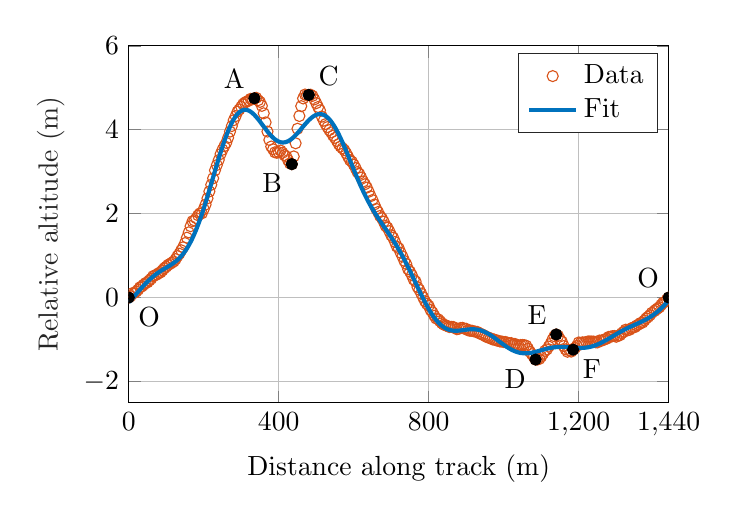
\begin{tikzpicture}[scale=1][]

  \begin{axis}[%
    width=2.7in,
    height=1.783in,
    at={(0.758in,2.6in)},
    scale only axis,
    xmin=0,
    xmax=1440,
    ymin=-2.5,
    ymax=6,
    ylabel style={font=\color{white!15!black}},
    ylabel={Relative altitude (\si{m})},
    xlabel={Distance along track (\si{m})},
    axis background/.style={fill=white},
    xmajorgrids,
    ymajorgrids,
    %xtick={0,350,700,1050,1440},
    xtick={0,400,800,1200,1440},
    clip marker paths=true,
    legend style={legend cell align=left, align=left, draw=white!15!black}
    ]
    \addplot [color=mycolor2, only marks, mark=o, mark options={solid, mycolor2}]
      table[row sep=crcr]{%
    0	0\\
    5.1222	0.035738\\
    10.052	0.10497\\
    15.102	0.10772\\
    20.056	0.14341\\
    25.018	0.18539\\
    30.099	0.24281\\
    35.019	0.26534\\
    40.103	0.30621\\
    45.03	0.34432\\
    50.02	0.36324\\
    55.06	0.4084\\
    60.082	0.44874\\
    65.003	0.50745\\
    70.013	0.52866\\
    75.043	0.54874\\
    80.029	0.58008\\
    85.054	0.60309\\
    90.004	0.64756\\
    95.034	0.69913\\
    100.08	0.73437\\
    105.09	0.77665\\
    110.03	0.80147\\
    115.11	0.8308\\
    120.05	0.85947\\
    125.08	0.91471\\
    130.04	0.987\\
    135.06	1.0446\\
    140.02	1.1265\\
    145.07	1.1976\\
    150.07	1.2977\\
    155.07	1.4261\\
    160.05	1.5534\\
    165.02	1.7003\\
    170.06	1.8176\\
    175.03	1.8384\\
    180.1	1.8899\\
    185.09	1.959\\
    190.08	2.0057\\
    195.07	2.0065\\
    200.08	2.1076\\
    205.05	2.2171\\
    210.04	2.3643\\
    215.1	2.5291\\
    220.07	2.6873\\
    225.1	2.8419\\
    230.05	3.0317\\
    235.08	3.1583\\
    240.02	3.2784\\
    245.01	3.4202\\
    250.02	3.5219\\
    255.05	3.6083\\
    260.01	3.6875\\
    265	3.8082\\
    270.07	3.9549\\
    275.02	4.0884\\
    280.08	4.2276\\
    285.07	4.3234\\
    290.09	4.4291\\
    295.02	4.4829\\
    300.06	4.5449\\
    305.07	4.61\\
    310.07	4.648\\
    315.05	4.6728\\
    320.01	4.6917\\
    325.05	4.7362\\
    330.01	4.7312\\
    335.08	4.7492\\
    340.01	4.7603\\
    345.05	4.7026\\
    350.06	4.6628\\
    355.04	4.5688\\
    360.09	4.3908\\
    365.05	4.1747\\
    370.01	3.9563\\
    375.05	3.7561\\
    380.01	3.5984\\
    385.01	3.5353\\
    390.02	3.4615\\
    395.07	3.4505\\
    400.1	3.4657\\
    405.04	3.5032\\
    410.05	3.4511\\
    415	3.3952\\
    420.07	3.3656\\
    425.01	3.2732\\
    430.02	3.1978\\
    435.03	3.1787\\
    440.06	3.3637\\
    445.07	3.6768\\
    450.11	4.0237\\
    455.11	4.3273\\
    460.03	4.5621\\
    465.01	4.7456\\
    470.09	4.8381\\
    475.01	4.8199\\
    480.09	4.8295\\
    485	4.8346\\
    490.09	4.8057\\
    495.09	4.7223\\
    500.09	4.6332\\
    505.1	4.5413\\
    510.02	4.4621\\
    515.05	4.3114\\
    520.05	4.2162\\
    525.01	4.134\\
    530.04	4.0624\\
    535.01	3.9909\\
    540	3.9346\\
    545.08	3.8595\\
    550.12	3.8051\\
    555.1	3.7335\\
    560.09	3.6563\\
    565.02	3.599\\
    570.06	3.5572\\
    575.09	3.5131\\
    580.08	3.4391\\
    585	3.3567\\
    590.01	3.2757\\
    595.05	3.2379\\
    600.02	3.1674\\
    605.08	3.0848\\
    610.02	2.9922\\
    615	2.9465\\
    620.02	2.8593\\
    625.11	2.7651\\
    630.08	2.6997\\
    635.08	2.6199\\
    640.02	2.5204\\
    645.04	2.4145\\
    650.07	2.3246\\
    655	2.2181\\
    660.06	2.1146\\
    665.02	2.038\\
    670.06	1.9449\\
    675.05	1.8925\\
    680.09	1.8092\\
    685.08	1.709\\
    690.04	1.6652\\
    695.04	1.5816\\
    700.02	1.4836\\
    705.1	1.4271\\
    710.02	1.3237\\
    715	1.2147\\
    720.11	1.1747\\
    725.08	1.0693\\
    730.02	0.9783\\
    735.02	0.87326\\
    740.01	0.80079\\
    745.06	0.67547\\
    750.09	0.61633\\
    755.06	0.53173\\
    760.08	0.42591\\
    765	0.38467\\
    770.1	0.25097\\
    775.04	0.185\\
    780.1	0.094467\\
    785.11	0.0042468\\
    790.01	-0.087749\\
    795.03	-0.15127\\
    800.04	-0.19791\\
    805.06	-0.29861\\
    810.07	-0.35415\\
    815.01	-0.43642\\
    820.07	-0.50071\\
    825.05	-0.5167\\
    830.08	-0.56259\\
    835.08	-0.6105\\
    840.01	-0.64431\\
    845.08	-0.66497\\
    850.11	-0.67766\\
    855.07	-0.70386\\
    860.02	-0.69959\\
    865.1	-0.70008\\
    870.02	-0.72612\\
    875.09	-0.75503\\
    880.11	-0.74512\\
    885.04	-0.72702\\
    890.06	-0.72219\\
    895.01	-0.74177\\
    900.04	-0.74645\\
    905.09	-0.78183\\
    910.06	-0.79228\\
    915.01	-0.79059\\
    920.11	-0.80498\\
    925	-0.81388\\
    930.09	-0.82108\\
    935.08	-0.85434\\
    940.08	-0.87037\\
    945.02	-0.8898\\
    950.11	-0.91711\\
    955	-0.941\\
    960.02	-0.95908\\
    965.01	-0.97259\\
    970.07	-0.9977\\
    975.02	-1.0021\\
    980.02	-1.0205\\
    985.06	-1.03\\
    990.07	-1.0475\\
    995.09	-1.0488\\
    1000.1	-1.0607\\
    1005	-1.0603\\
    1010.1	-1.0762\\
    1015	-1.0899\\
    1020.1	-1.0865\\
    1025	-1.1233\\
    1030	-1.1057\\
    1035.1	-1.1309\\
    1040.1	-1.1516\\
    1045.1	-1.1333\\
    1050.1	-1.1306\\
    1055	-1.1343\\
    1060.1	-1.1496\\
    1065	-1.2185\\
    1070.1	-1.294\\
    1075.1	-1.3496\\
    1080.1	-1.4133\\
    1085.1	-1.4789\\
    1090.1	-1.4778\\
    1095.1	-1.4619\\
    1100	-1.4065\\
    1105	-1.3362\\
    1110.1	-1.2712\\
    1115.1	-1.2374\\
    1120.1	-1.1685\\
    1125.1	-1.0986\\
    1130	-1.0041\\
    1135	-0.92332\\
    1140	-0.88023\\
    1145.1	-0.91493\\
    1150.1	-0.9995\\
    1155	-1.0491\\
    1160.1	-1.1572\\
    1165	-1.2352\\
    1170.1	-1.2925\\
    1175	-1.2543\\
    1180.1	-1.2889\\
    1185.1	-1.2424\\
    1190.1	-1.2007\\
    1195	-1.1524\\
    1200.1	-1.0711\\
    1205	-1.0818\\
    1210	-1.0683\\
    1215.1	-1.0743\\
    1220	-1.0607\\
    1225	-1.0466\\
    1230.1	-1.0469\\
    1235.1	-1.049\\
    1240	-1.0506\\
    1245	-1.0674\\
    1250	-1.0704\\
    1255.1	-1.0248\\
    1260.1	-1.0326\\
    1265	-1.0105\\
    1270.1	-0.99422\\
    1275	-0.98019\\
    1280.1	-0.93839\\
    1285	-0.93409\\
    1290.1	-0.92035\\
    1295.1	-0.9174\\
    1300	-0.93492\\
    1305.1	-0.91239\\
    1310.1	-0.89661\\
    1315.1	-0.85047\\
    1320.1	-0.81659\\
    1325.1	-0.76624\\
    1330.1	-0.78241\\
    1335	-0.77116\\
    1340.1	-0.73442\\
    1345.1	-0.71422\\
    1350	-0.70423\\
    1355	-0.66556\\
    1360.1	-0.63987\\
    1365.1	-0.60605\\
    1370	-0.59789\\
    1375	-0.54782\\
    1380	-0.49583\\
    1385	-0.46034\\
    1390	-0.41838\\
    1395.1	-0.363\\
    1401.9	-0.32049\\
    1406.3	-0.28726\\
    1410.6	-0.25818\\
    1415.1	-0.22964\\
    1420	-0.17512\\
    1425	-0.12472\\
    1430.1	-0.10287\\
    1435.1	-0.048184\\
    1440	-0.01308\\
    1440	0\\
    1445.1222	0.035738\\
    1450.052	0.10497\\
    1455.102	0.10772\\
    1460.056	0.14341\\
    1465.018	0.18539\\
    1470.099	0.24281\\
    1475.019	0.26534\\
    1480.103	0.30621\\
    1485.03	0.34432\\
    1490.02	0.36324\\
    1495.06	0.4084\\
    1500.082	0.44874\\
    1505.003	0.50745\\
    1510.013	0.52866\\
    1515.043	0.54874\\
    1520.029	0.58008\\
    1525.054	0.60309\\
    1530.004	0.64756\\
    1535.034	0.69913\\
    1540.08	0.73437\\
    1545.09	0.77665\\
    1550.03	0.80147\\
    1555.11	0.8308\\
    1560.05	0.85947\\
    1565.08	0.91471\\
    1570.04	0.987\\
    1575.06	1.0446\\
    1580.02	1.1265\\
    1585.07	1.1976\\
    1590.07	1.2977\\
    1595.07	1.4261\\
    1600.05	1.5534\\
    1605.02	1.7003\\
    1610.06	1.8176\\
    1615.03	1.8384\\
    1620.1	1.8899\\
    1625.09	1.959\\
    1630.08	2.0057\\
    1635.07	2.0065\\
    1640.08	2.1076\\
    1645.05	2.2171\\
    1650.04	2.3643\\
    1655.1	2.5291\\
    1660.07	2.6873\\
    1665.1	2.8419\\
    1670.05	3.0317\\
    1675.08	3.1583\\
    1680.02	3.2784\\
    1685.01	3.4202\\
    1690.02	3.5219\\
    1695.05	3.6083\\
    1700.01	3.6875\\
    1705	3.8082\\
    1710.07	3.9549\\
    1715.02	4.0884\\
    1720.08	4.2276\\
    1725.07	4.3234\\
    1730.09	4.4291\\
    1735.02	4.4829\\
    1740.06	4.5449\\
    1745.07	4.61\\
    1750.07	4.648\\
    1755.05	4.6728\\
    1760.01	4.6917\\
    1765.05	4.7362\\
    1770.01	4.7312\\
    1775.08	4.7492\\
    1780.01	4.7603\\
    1785.05	4.7026\\
    1790.06	4.6628\\
    1795.04	4.5688\\
    1800.09	4.3908\\
    1805.05	4.1747\\
    1810.01	3.9563\\
    1815.05	3.7561\\
    1820.01	3.5984\\
    1825.01	3.5353\\
    1830.02	3.4615\\
    1835.07	3.4505\\
    1840.1	3.4657\\
    1845.04	3.5032\\
    1850.05	3.4511\\
    1855	3.3952\\
    1860.07	3.3656\\
    1865.01	3.2732\\
    1870.02	3.1978\\
    1875.03	3.1787\\
    1880.06	3.3637\\
    1885.07	3.6768\\
    1890.11	4.0237\\
    1895.11	4.3273\\
    1900.03	4.5621\\
    1905.01	4.7456\\
    1910.09	4.8381\\
    1915.01	4.8199\\
    1920.09	4.8295\\
    1925	4.8346\\
    1930.09	4.8057\\
    1935.09	4.7223\\
    1940.09	4.6332\\
    1945.1	4.5413\\
    1950.02	4.4621\\
    1955.05	4.3114\\
    1960.05	4.2162\\
    1965.01	4.134\\
    1970.04	4.0624\\
    1975.01	3.9909\\
    1980	3.9346\\
    1985.08	3.8595\\
    1990.12	3.8051\\
    1995.1	3.7335\\
    2000.09	3.6563\\
    2005.02	3.599\\
    2010.06	3.5572\\
    2015.09	3.5131\\
    2020.08	3.4391\\
    2025	3.3567\\
    2030.01	3.2757\\
    2035.05	3.2379\\
    2040.02	3.1674\\
    2045.08	3.0848\\
    2050.02	2.9922\\
    2055	2.9465\\
    2060.02	2.8593\\
    2065.11	2.7651\\
    2070.08	2.6997\\
    2075.08	2.6199\\
    2080.02	2.5204\\
    2085.04	2.4145\\
    2090.07	2.3246\\
    2095	2.2181\\
    2100.06	2.1146\\
    2105.02	2.038\\
    2110.06	1.9449\\
    2115.05	1.8925\\
    2120.09	1.8092\\
    2125.08	1.709\\
    2130.04	1.6652\\
    2135.04	1.5816\\
    2140.02	1.4836\\
    2145.1	1.4271\\
    2150.02	1.3237\\
    2155	1.2147\\
    2160.11	1.1747\\
    2165.08	1.0693\\
    2170.02	0.9783\\
    2175.02	0.87326\\
    2180.01	0.80079\\
    2185.06	0.67547\\
    2190.09	0.61633\\
    2195.06	0.53173\\
    2200.08	0.42591\\
    2205	0.38467\\
    2210.1	0.25097\\
    2215.04	0.185\\
    2220.1	0.094467\\
    2225.11	0.0042468\\
    2230.01	-0.087749\\
    2235.03	-0.15127\\
    2240.04	-0.19791\\
    2245.06	-0.29861\\
    2250.07	-0.35415\\
    2255.01	-0.43642\\
    2260.07	-0.50071\\
    2265.05	-0.5167\\
    2270.08	-0.56259\\
    2275.08	-0.6105\\
    2280.01	-0.64431\\
    2285.08	-0.66497\\
    2290.11	-0.67766\\
    2295.07	-0.70386\\
    2300.02	-0.69959\\
    2305.1	-0.70008\\
    2310.02	-0.72612\\
    2315.09	-0.75503\\
    2320.11	-0.74512\\
    2325.04	-0.72702\\
    2330.06	-0.72219\\
    2335.01	-0.74177\\
    2340.04	-0.74645\\
    2345.09	-0.78183\\
    2350.06	-0.79228\\
    2355.01	-0.79059\\
    2360.11	-0.80498\\
    2365	-0.81388\\
    2370.09	-0.82108\\
    2375.08	-0.85434\\
    2380.08	-0.87037\\
    2385.02	-0.8898\\
    2390.11	-0.91711\\
    2395	-0.941\\
    2400.02	-0.95908\\
    2405.01	-0.97259\\
    2410.07	-0.9977\\
    2415.02	-1.0021\\
    2420.02	-1.0205\\
    2425.06	-1.03\\
    2430.07	-1.0475\\
    2435.09	-1.0488\\
    2440.1	-1.0607\\
    2445	-1.0603\\
    2450.1	-1.0762\\
    2455	-1.0899\\
    2460.1	-1.0865\\
    2465	-1.1233\\
    2470	-1.1057\\
    2475.1	-1.1309\\
    2480.1	-1.1516\\
    2485.1	-1.1333\\
    2490.1	-1.1306\\
    2495	-1.1343\\
    2500.1	-1.1496\\
    2505	-1.2185\\
    2510.1	-1.294\\
    2515.1	-1.3496\\
    2520.1	-1.4133\\
    2525.1	-1.4789\\
    2530.1	-1.4778\\
    2535.1	-1.4619\\
    2540	-1.4065\\
    2545	-1.3362\\
    2550.1	-1.2712\\
    2555.1	-1.2374\\
    2560.1	-1.1685\\
    2565.1	-1.0986\\
    2570	-1.0041\\
    2575	-0.92332\\
    2580	-0.88023\\
    2585.1	-0.91493\\
    2590.1	-0.9995\\
    2595	-1.0491\\
    2600.1	-1.1572\\
    2605	-1.2352\\
    2610.1	-1.2925\\
    2615	-1.2543\\
    2620.1	-1.2889\\
    2625.1	-1.2424\\
    2630.1	-1.2007\\
    2635	-1.1524\\
    2640.1	-1.0711\\
    2645	-1.0818\\
    2650	-1.0683\\
    2655.1	-1.0743\\
    2660	-1.0607\\
    2665	-1.0466\\
    2670.1	-1.0469\\
    2675.1	-1.049\\
    2680	-1.0506\\
    2685	-1.0674\\
    2690	-1.0704\\
    2695.1	-1.0248\\
    2700.1	-1.0326\\
    2705	-1.0105\\
    2710.1	-0.99422\\
    2715	-0.98019\\
    2720.1	-0.93839\\
    2725	-0.93409\\
    2730.1	-0.92035\\
    2735.1	-0.9174\\
    2740	-0.93492\\
    2745.1	-0.91239\\
    2750.1	-0.89661\\
    2755.1	-0.85047\\
    2760.1	-0.81659\\
    2765.1	-0.76624\\
    2770.1	-0.78241\\
    2775	-0.77116\\
    2780.1	-0.73442\\
    2785.1	-0.71422\\
    2790	-0.70423\\
    2795	-0.66556\\
    2800.1	-0.63987\\
    2805.1	-0.60605\\
    2810	-0.59789\\
    2815	-0.54782\\
    2820	-0.49583\\
    2825	-0.46034\\
    2830	-0.41838\\
    2835.1	-0.363\\
    2841.9	-0.32049\\
    2846.3	-0.28726\\
    2850.6	-0.25818\\
    2855.1	-0.22964\\
    2860	-0.17512\\
    2865	-0.12472\\
    2870.1	-0.10287\\
    2875.1	-0.048184\\
    2880	-0.01308\\
    2880	0\\
    2885.1222	0.035738\\
    2890.052	0.10497\\
    2895.102	0.10772\\
    2900.056	0.14341\\
    2905.018	0.18539\\
    2910.099	0.24281\\
    2915.019	0.26534\\
    2920.103	0.30621\\
    2925.03	0.34432\\
    2930.02	0.36324\\
    2935.06	0.4084\\
    2940.082	0.44874\\
    2945.003	0.50745\\
    2950.013	0.52866\\
    2955.043	0.54874\\
    2960.029	0.58008\\
    2965.054	0.60309\\
    2970.004	0.64756\\
    2975.034	0.69913\\
    2980.08	0.73437\\
    2985.09	0.77665\\
    2990.03	0.80147\\
    2995.11	0.8308\\
    3000.05	0.85947\\
    3005.08	0.91471\\
    3010.04	0.987\\
    3015.06	1.0446\\
    3020.02	1.1265\\
    3025.07	1.1976\\
    3030.07	1.2977\\
    3035.07	1.4261\\
    3040.05	1.5534\\
    3045.02	1.7003\\
    3050.06	1.8176\\
    3055.03	1.8384\\
    3060.1	1.8899\\
    3065.09	1.959\\
    3070.08	2.0057\\
    3075.07	2.0065\\
    3080.08	2.1076\\
    3085.05	2.2171\\
    3090.04	2.3643\\
    3095.1	2.5291\\
    3100.07	2.6873\\
    3105.1	2.8419\\
    3110.05	3.0317\\
    3115.08	3.1583\\
    3120.02	3.2784\\
    3125.01	3.4202\\
    3130.02	3.5219\\
    3135.05	3.6083\\
    3140.01	3.6875\\
    3145	3.8082\\
    3150.07	3.9549\\
    3155.02	4.0884\\
    3160.08	4.2276\\
    3165.07	4.3234\\
    3170.09	4.4291\\
    3175.02	4.4829\\
    3180.06	4.5449\\
    3185.07	4.61\\
    3190.07	4.648\\
    3195.05	4.6728\\
    3200.01	4.6917\\
    3205.05	4.7362\\
    3210.01	4.7312\\
    3215.08	4.7492\\
    3220.01	4.7603\\
    3225.05	4.7026\\
    3230.06	4.6628\\
    3235.04	4.5688\\
    3240.09	4.3908\\
    3245.05	4.1747\\
    3250.01	3.9563\\
    3255.05	3.7561\\
    3260.01	3.5984\\
    3265.01	3.5353\\
    3270.02	3.4615\\
    3275.07	3.4505\\
    3280.1	3.4657\\
    3285.04	3.5032\\
    3290.05	3.4511\\
    3295	3.3952\\
    3300.07	3.3656\\
    3305.01	3.2732\\
    3310.02	3.1978\\
    3315.03	3.1787\\
    3320.06	3.3637\\
    3325.07	3.6768\\
    3330.11	4.0237\\
    3335.11	4.3273\\
    3340.03	4.5621\\
    3345.01	4.7456\\
    3350.09	4.8381\\
    3355.01	4.8199\\
    3360.09	4.8295\\
    3365	4.8346\\
    3370.09	4.8057\\
    3375.09	4.7223\\
    3380.09	4.6332\\
    3385.1	4.5413\\
    3390.02	4.4621\\
    3395.05	4.3114\\
    3400.05	4.2162\\
    3405.01	4.134\\
    3410.04	4.0624\\
    3415.01	3.9909\\
    3420	3.9346\\
    3425.08	3.8595\\
    3430.12	3.8051\\
    3435.1	3.7335\\
    3440.09	3.6563\\
    3445.02	3.599\\
    3450.06	3.5572\\
    3455.09	3.5131\\
    3460.08	3.4391\\
    3465	3.3567\\
    3470.01	3.2757\\
    3475.05	3.2379\\
    3480.02	3.1674\\
    3485.08	3.0848\\
    3490.02	2.9922\\
    3495	2.9465\\
    3500.02	2.8593\\
    3505.11	2.7651\\
    3510.08	2.6997\\
    3515.08	2.6199\\
    3520.02	2.5204\\
    3525.04	2.4145\\
    3530.07	2.3246\\
    3535	2.2181\\
    3540.06	2.1146\\
    3545.02	2.038\\
    3550.06	1.9449\\
    3555.05	1.8925\\
    3560.09	1.8092\\
    3565.08	1.709\\
    3570.04	1.6652\\
    3575.04	1.5816\\
    3580.02	1.4836\\
    3585.1	1.4271\\
    3590.02	1.3237\\
    3595	1.2147\\
    3600.11	1.1747\\
    3605.08	1.0693\\
    3610.02	0.9783\\
    3615.02	0.87326\\
    3620.01	0.80079\\
    3625.06	0.67547\\
    3630.09	0.61633\\
    3635.06	0.53173\\
    3640.08	0.42591\\
    3645	0.38467\\
    3650.1	0.25097\\
    3655.04	0.185\\
    3660.1	0.094467\\
    3665.11	0.0042468\\
    3670.01	-0.087749\\
    3675.03	-0.15127\\
    3680.04	-0.19791\\
    3685.06	-0.29861\\
    3690.07	-0.35415\\
    3695.01	-0.43642\\
    3700.07	-0.50071\\
    3705.05	-0.5167\\
    3710.08	-0.56259\\
    3715.08	-0.6105\\
    3720.01	-0.64431\\
    3725.08	-0.66497\\
    3730.11	-0.67766\\
    3735.07	-0.70386\\
    3740.02	-0.69959\\
    3745.1	-0.70008\\
    3750.02	-0.72612\\
    3755.09	-0.75503\\
    3760.11	-0.74512\\
    3765.04	-0.72702\\
    3770.06	-0.72219\\
    3775.01	-0.74177\\
    3780.04	-0.74645\\
    3785.09	-0.78183\\
    3790.06	-0.79228\\
    3795.01	-0.79059\\
    3800.11	-0.80498\\
    3805	-0.81388\\
    3810.09	-0.82108\\
    3815.08	-0.85434\\
    3820.08	-0.87037\\
    3825.02	-0.8898\\
    3830.11	-0.91711\\
    3835	-0.941\\
    3840.02	-0.95908\\
    3845.01	-0.97259\\
    3850.07	-0.9977\\
    3855.02	-1.0021\\
    3860.02	-1.0205\\
    3865.06	-1.03\\
    3870.07	-1.0475\\
    3875.09	-1.0488\\
    3880.1	-1.0607\\
    3885	-1.0603\\
    3890.1	-1.0762\\
    3895	-1.0899\\
    3900.1	-1.0865\\
    3905	-1.1233\\
    3910	-1.1057\\
    3915.1	-1.1309\\
    3920.1	-1.1516\\
    3925.1	-1.1333\\
    3930.1	-1.1306\\
    3935	-1.1343\\
    3940.1	-1.1496\\
    3945	-1.2185\\
    3950.1	-1.294\\
    3955.1	-1.3496\\
    3960.1	-1.4133\\
    3965.1	-1.4789\\
    3970.1	-1.4778\\
    3975.1	-1.4619\\
    3980	-1.4065\\
    3985	-1.3362\\
    3990.1	-1.2712\\
    3995.1	-1.2374\\
    4000.1	-1.1685\\
    4005.1	-1.0986\\
    4010	-1.0041\\
    4015	-0.92332\\
    4020	-0.88023\\
    4025.1	-0.91493\\
    4030.1	-0.9995\\
    4035	-1.0491\\
    4040.1	-1.1572\\
    4045	-1.2352\\
    4050.1	-1.2925\\
    4055	-1.2543\\
    4060.1	-1.2889\\
    4065.1	-1.2424\\
    4070.1	-1.2007\\
    4075	-1.1524\\
    4080.1	-1.0711\\
    4085	-1.0818\\
    4090	-1.0683\\
    4095.1	-1.0743\\
    4100	-1.0607\\
    4105	-1.0466\\
    4110.1	-1.0469\\
    4115.1	-1.049\\
    4120	-1.0506\\
    4125	-1.0674\\
    4130	-1.0704\\
    4135.1	-1.0248\\
    4140.1	-1.0326\\
    4145	-1.0105\\
    4150.1	-0.99422\\
    4155	-0.98019\\
    4160.1	-0.93839\\
    4165	-0.93409\\
    4170.1	-0.92035\\
    4175.1	-0.9174\\
    4180	-0.93492\\
    4185.1	-0.91239\\
    4190.1	-0.89661\\
    4195.1	-0.85047\\
    4200.1	-0.81659\\
    4205.1	-0.76624\\
    4210.1	-0.78241\\
    4215	-0.77116\\
    4220.1	-0.73442\\
    4225.1	-0.71422\\
    4230	-0.70423\\
    4235	-0.66556\\
    4240.1	-0.63987\\
    4245.1	-0.60605\\
    4250	-0.59789\\
    4255	-0.54782\\
    4260	-0.49583\\
    4265	-0.46034\\
    4270	-0.41838\\
    4275.1	-0.363\\
    4281.9	-0.32049\\
    4286.3	-0.28726\\
    4290.6	-0.25818\\
    4295.1	-0.22964\\
    4300	-0.17512\\
    4305	-0.12472\\
    4310.1	-0.10287\\
    4315.1	-0.048184\\
    4320	-0.01308\\
    4320	0\\
    4325.1222	0.035738\\
    4330.052	0.10497\\
    4335.102	0.10772\\
    4340.056	0.14341\\
    4345.018	0.18539\\
    4350.099	0.24281\\
    4355.019	0.26534\\
    4360.103	0.30621\\
    4365.03	0.34432\\
    4370.02	0.36324\\
    4375.06	0.4084\\
    4380.082	0.44874\\
    4385.003	0.50745\\
    4390.013	0.52866\\
    4395.043	0.54874\\
    4400.029	0.58008\\
    4405.054	0.60309\\
    4410.004	0.64756\\
    4415.034	0.69913\\
    4420.08	0.73437\\
    4425.09	0.77665\\
    4430.03	0.80147\\
    4435.11	0.8308\\
    4440.05	0.85947\\
    4445.08	0.91471\\
    4450.04	0.987\\
    4455.06	1.0446\\
    4460.02	1.1265\\
    4465.07	1.1976\\
    4470.07	1.2977\\
    4475.07	1.4261\\
    4480.05	1.5534\\
    4485.02	1.7003\\
    4490.06	1.8176\\
    4495.03	1.8384\\
    4500.1	1.8899\\
    4505.09	1.959\\
    4510.08	2.0057\\
    4515.07	2.0065\\
    4520.08	2.1076\\
    4525.05	2.2171\\
    4530.04	2.3643\\
    4535.1	2.5291\\
    4540.07	2.6873\\
    4545.1	2.8419\\
    4550.05	3.0317\\
    4555.08	3.1583\\
    4560.02	3.2784\\
    4565.01	3.4202\\
    4570.02	3.5219\\
    4575.05	3.6083\\
    4580.01	3.6875\\
    4585	3.8082\\
    4590.07	3.9549\\
    4595.02	4.0884\\
    4600.08	4.2276\\
    4605.07	4.3234\\
    4610.09	4.4291\\
    4615.02	4.4829\\
    4620.06	4.5449\\
    4625.07	4.61\\
    4630.07	4.648\\
    4635.05	4.6728\\
    4640.01	4.6917\\
    4645.05	4.7362\\
    4650.01	4.7312\\
    4655.08	4.7492\\
    4660.01	4.7603\\
    4665.05	4.7026\\
    4670.06	4.6628\\
    4675.04	4.5688\\
    4680.09	4.3908\\
    4685.05	4.1747\\
    4690.01	3.9563\\
    4695.05	3.7561\\
    4700.01	3.5984\\
    4705.01	3.5353\\
    4710.02	3.4615\\
    4715.07	3.4505\\
    4720.1	3.4657\\
    4725.04	3.5032\\
    4730.05	3.4511\\
    4735	3.3952\\
    4740.07	3.3656\\
    4745.01	3.2732\\
    4750.02	3.1978\\
    4755.03	3.1787\\
    4760.06	3.3637\\
    4765.07	3.6768\\
    4770.11	4.0237\\
    4775.11	4.3273\\
    4780.03	4.5621\\
    4785.01	4.7456\\
    4790.09	4.8381\\
    4795.01	4.8199\\
    4800.09	4.8295\\
    4805	4.8346\\
    4810.09	4.8057\\
    4815.09	4.7223\\
    4820.09	4.6332\\
    4825.1	4.5413\\
    4830.02	4.4621\\
    4835.05	4.3114\\
    4840.05	4.2162\\
    4845.01	4.134\\
    4850.04	4.0624\\
    4855.01	3.9909\\
    4860	3.9346\\
    4865.08	3.8595\\
    4870.12	3.8051\\
    4875.1	3.7335\\
    4880.09	3.6563\\
    4885.02	3.599\\
    4890.06	3.5572\\
    4895.09	3.5131\\
    4900.08	3.4391\\
    4905	3.3567\\
    4910.01	3.2757\\
    4915.05	3.2379\\
    4920.02	3.1674\\
    4925.08	3.0848\\
    4930.02	2.9922\\
    4935	2.9465\\
    4940.02	2.8593\\
    4945.11	2.7651\\
    4950.08	2.6997\\
    4955.08	2.6199\\
    4960.02	2.5204\\
    4965.04	2.4145\\
    4970.07	2.3246\\
    4975	2.2181\\
    4980.06	2.1146\\
    4985.02	2.038\\
    4990.06	1.9449\\
    4995.05	1.8925\\
    5000.09	1.8092\\
    5005.08	1.709\\
    5010.04	1.6652\\
    5015.04	1.5816\\
    5020.02	1.4836\\
    5025.1	1.4271\\
    5030.02	1.3237\\
    5035	1.2147\\
    5040.11	1.1747\\
    5045.08	1.0693\\
    5050.02	0.9783\\
    5055.02	0.87326\\
    5060.01	0.80079\\
    5065.06	0.67547\\
    5070.09	0.61633\\
    5075.06	0.53173\\
    5080.08	0.42591\\
    5085	0.38467\\
    5090.1	0.25097\\
    5095.04	0.185\\
    5100.1	0.094467\\
    5105.11	0.0042468\\
    5110.01	-0.087749\\
    5115.03	-0.15127\\
    5120.04	-0.19791\\
    5125.06	-0.29861\\
    5130.07	-0.35415\\
    5135.01	-0.43642\\
    5140.07	-0.50071\\
    5145.05	-0.5167\\
    5150.08	-0.56259\\
    5155.08	-0.6105\\
    5160.01	-0.64431\\
    5165.08	-0.66497\\
    5170.11	-0.67766\\
    5175.07	-0.70386\\
    5180.02	-0.69959\\
    5185.1	-0.70008\\
    5190.02	-0.72612\\
    5195.09	-0.75503\\
    5200.11	-0.74512\\
    5205.04	-0.72702\\
    5210.06	-0.72219\\
    5215.01	-0.74177\\
    5220.04	-0.74645\\
    5225.09	-0.78183\\
    5230.06	-0.79228\\
    5235.01	-0.79059\\
    5240.11	-0.80498\\
    5245	-0.81388\\
    5250.09	-0.82108\\
    5255.08	-0.85434\\
    5260.08	-0.87037\\
    5265.02	-0.8898\\
    5270.11	-0.91711\\
    5275	-0.941\\
    5280.02	-0.95908\\
    5285.01	-0.97259\\
    5290.07	-0.9977\\
    5295.02	-1.0021\\
    5300.02	-1.0205\\
    5305.06	-1.03\\
    5310.07	-1.0475\\
    5315.09	-1.0488\\
    5320.1	-1.0607\\
    5325	-1.0603\\
    5330.1	-1.0762\\
    5335	-1.0899\\
    5340.1	-1.0865\\
    5345	-1.1233\\
    5350	-1.1057\\
    5355.1	-1.1309\\
    5360.1	-1.1516\\
    5365.1	-1.1333\\
    5370.1	-1.1306\\
    5375	-1.1343\\
    5380.1	-1.1496\\
    5385	-1.2185\\
    5390.1	-1.294\\
    5395.1	-1.3496\\
    5400.1	-1.4133\\
    5405.1	-1.4789\\
    5410.1	-1.4778\\
    5415.1	-1.4619\\
    5420	-1.4065\\
    5425	-1.3362\\
    5430.1	-1.2712\\
    5435.1	-1.2374\\
    5440.1	-1.1685\\
    5445.1	-1.0986\\
    5450	-1.0041\\
    5455	-0.92332\\
    5460	-0.88023\\
    5465.1	-0.91493\\
    5470.1	-0.9995\\
    5475	-1.0491\\
    5480.1	-1.1572\\
    5485	-1.2352\\
    5490.1	-1.2925\\
    5495	-1.2543\\
    5500.1	-1.2889\\
    5505.1	-1.2424\\
    5510.1	-1.2007\\
    5515	-1.1524\\
    5520.1	-1.0711\\
    5525	-1.0818\\
    5530	-1.0683\\
    5535.1	-1.0743\\
    5540	-1.0607\\
    5545	-1.0466\\
    5550.1	-1.0469\\
    5555.1	-1.049\\
    5560	-1.0506\\
    5565	-1.0674\\
    5570	-1.0704\\
    5575.1	-1.0248\\
    5580.1	-1.0326\\
    5585	-1.0105\\
    5590.1	-0.99422\\
    5595	-0.98019\\
    5600.1	-0.93839\\
    5605	-0.93409\\
    5610.1	-0.92035\\
    5615.1	-0.9174\\
    5620	-0.93492\\
    5625.1	-0.91239\\
    5630.1	-0.89661\\
    5635.1	-0.85047\\
    5640.1	-0.81659\\
    5645.1	-0.76624\\
    5650.1	-0.78241\\
    5655	-0.77116\\
    5660.1	-0.73442\\
    5665.1	-0.71422\\
    5670	-0.70423\\
    5675	-0.66556\\
    5680.1	-0.63987\\
    5685.1	-0.60605\\
    5690	-0.59789\\
    5695	-0.54782\\
    5700	-0.49583\\
    5705	-0.46034\\
    5710	-0.41838\\
    5715.1	-0.363\\
    5721.9	-0.32049\\
    5726.3	-0.28726\\
    5730.6	-0.25818\\
    5735.1	-0.22964\\
    5740	-0.17512\\
    5745	-0.12472\\
    5750.1	-0.10287\\
    5755.1	-0.048184\\
    5760	-0.01308\\
    5760	0\\
    5765.1222	0.035738\\
    5770.052	0.10497\\
    5775.102	0.10772\\
    5780.056	0.14341\\
    5785.018	0.18539\\
    5790.099	0.24281\\
    5795.019	0.26534\\
    5800.103	0.30621\\
    5805.03	0.34432\\
    5810.02	0.36324\\
    5815.06	0.4084\\
    5820.082	0.44874\\
    5825.003	0.50745\\
    5830.013	0.52866\\
    5835.043	0.54874\\
    5840.029	0.58008\\
    5845.054	0.60309\\
    5850.004	0.64756\\
    5855.034	0.69913\\
    5860.08	0.73437\\
    5865.09	0.77665\\
    5870.03	0.80147\\
    5875.11	0.8308\\
    5880.05	0.85947\\
    5885.08	0.91471\\
    5890.04	0.987\\
    5895.06	1.0446\\
    5900.02	1.1265\\
    5905.07	1.1976\\
    5910.07	1.2977\\
    5915.07	1.4261\\
    5920.05	1.5534\\
    5925.02	1.7003\\
    5930.06	1.8176\\
    5935.03	1.8384\\
    5940.1	1.8899\\
    5945.09	1.959\\
    5950.08	2.0057\\
    5955.07	2.0065\\
    5960.08	2.1076\\
    5965.05	2.2171\\
    5970.04	2.3643\\
    5975.1	2.5291\\
    5980.07	2.6873\\
    5985.1	2.8419\\
    5990.05	3.0317\\
    5995.08	3.1583\\
    6000.02	3.2784\\
    6005.01	3.4202\\
    6010.02	3.5219\\
    6015.05	3.6083\\
    6020.01	3.6875\\
    6025	3.8082\\
    6030.07	3.9549\\
    6035.02	4.0884\\
    6040.08	4.2276\\
    6045.07	4.3234\\
    6050.09	4.4291\\
    6055.02	4.4829\\
    6060.06	4.5449\\
    6065.07	4.61\\
    6070.07	4.648\\
    6075.05	4.6728\\
    6080.01	4.6917\\
    6085.05	4.7362\\
    6090.01	4.7312\\
    6095.08	4.7492\\
    6100.01	4.7603\\
    6105.05	4.7026\\
    6110.06	4.6628\\
    6115.04	4.5688\\
    6120.09	4.3908\\
    6125.05	4.1747\\
    6130.01	3.9563\\
    6135.05	3.7561\\
    6140.01	3.5984\\
    6145.01	3.5353\\
    6150.02	3.4615\\
    6155.07	3.4505\\
    6160.1	3.4657\\
    6165.04	3.5032\\
    6170.05	3.4511\\
    6175	3.3952\\
    6180.07	3.3656\\
    6185.01	3.2732\\
    6190.02	3.1978\\
    6195.03	3.1787\\
    6200.06	3.3637\\
    6205.07	3.6768\\
    6210.11	4.0237\\
    6215.11	4.3273\\
    6220.03	4.5621\\
    6225.01	4.7456\\
    6230.09	4.8381\\
    6235.01	4.8199\\
    6240.09	4.8295\\
    6245	4.8346\\
    6250.09	4.8057\\
    6255.09	4.7223\\
    6260.09	4.6332\\
    6265.1	4.5413\\
    6270.02	4.4621\\
    6275.05	4.3114\\
    6280.05	4.2162\\
    6285.01	4.134\\
    6290.04	4.0624\\
    6295.01	3.9909\\
    6300	3.9346\\
    6305.08	3.8595\\
    6310.12	3.8051\\
    6315.1	3.7335\\
    6320.09	3.6563\\
    6325.02	3.599\\
    6330.06	3.5572\\
    6335.09	3.5131\\
    6340.08	3.4391\\
    6345	3.3567\\
    6350.01	3.2757\\
    6355.05	3.2379\\
    6360.02	3.1674\\
    6365.08	3.0848\\
    6370.02	2.9922\\
    6375	2.9465\\
    6380.02	2.8593\\
    6385.11	2.7651\\
    6390.08	2.6997\\
    6395.08	2.6199\\
    6400.02	2.5204\\
    6405.04	2.4145\\
    6410.07	2.3246\\
    6415	2.2181\\
    6420.06	2.1146\\
    6425.02	2.038\\
    6430.06	1.9449\\
    6435.05	1.8925\\
    6440.09	1.8092\\
    6445.08	1.709\\
    6450.04	1.6652\\
    6455.04	1.5816\\
    6460.02	1.4836\\
    6465.1	1.4271\\
    6470.02	1.3237\\
    6475	1.2147\\
    6480.11	1.1747\\
    6485.08	1.0693\\
    6490.02	0.9783\\
    6495.02	0.87326\\
    6500.01	0.80079\\
    6505.06	0.67547\\
    6510.09	0.61633\\
    6515.06	0.53173\\
    6520.08	0.42591\\
    6525	0.38467\\
    6530.1	0.25097\\
    6535.04	0.185\\
    6540.1	0.094467\\
    6545.11	0.0042468\\
    6550.01	-0.087749\\
    6555.03	-0.15127\\
    6560.04	-0.19791\\
    6565.06	-0.29861\\
    6570.07	-0.35415\\
    6575.01	-0.43642\\
    6580.07	-0.50071\\
    6585.05	-0.5167\\
    6590.08	-0.56259\\
    6595.08	-0.6105\\
    6600.01	-0.64431\\
    6605.08	-0.66497\\
    6610.11	-0.67766\\
    6615.07	-0.70386\\
    6620.02	-0.69959\\
    6625.1	-0.70008\\
    6630.02	-0.72612\\
    6635.09	-0.75503\\
    6640.11	-0.74512\\
    6645.04	-0.72702\\
    6650.06	-0.72219\\
    6655.01	-0.74177\\
    6660.04	-0.74645\\
    6665.09	-0.78183\\
    6670.06	-0.79228\\
    6675.01	-0.79059\\
    6680.11	-0.80498\\
    6685	-0.81388\\
    6690.09	-0.82108\\
    6695.08	-0.85434\\
    6700.08	-0.87037\\
    6705.02	-0.8898\\
    6710.11	-0.91711\\
    6715	-0.941\\
    6720.02	-0.95908\\
    6725.01	-0.97259\\
    6730.07	-0.9977\\
    6735.02	-1.0021\\
    6740.02	-1.0205\\
    6745.06	-1.03\\
    6750.07	-1.0475\\
    6755.09	-1.0488\\
    6760.1	-1.0607\\
    6765	-1.0603\\
    6770.1	-1.0762\\
    6775	-1.0899\\
    6780.1	-1.0865\\
    6785	-1.1233\\
    6790	-1.1057\\
    6795.1	-1.1309\\
    6800.1	-1.1516\\
    6805.1	-1.1333\\
    6810.1	-1.1306\\
    6815	-1.1343\\
    6820.1	-1.1496\\
    6825	-1.2185\\
    6830.1	-1.294\\
    6835.1	-1.3496\\
    6840.1	-1.4133\\
    6845.1	-1.4789\\
    6850.1	-1.4778\\
    6855.1	-1.4619\\
    6860	-1.4065\\
    6865	-1.3362\\
    6870.1	-1.2712\\
    6875.1	-1.2374\\
    6880.1	-1.1685\\
    6885.1	-1.0986\\
    6890	-1.0041\\
    6895	-0.92332\\
    6900	-0.88023\\
    6905.1	-0.91493\\
    6910.1	-0.9995\\
    6915	-1.0491\\
    6920.1	-1.1572\\
    6925	-1.2352\\
    6930.1	-1.2925\\
    6935	-1.2543\\
    6940.1	-1.2889\\
    6945.1	-1.2424\\
    6950.1	-1.2007\\
    6955	-1.1524\\
    6960.1	-1.0711\\
    6965	-1.0818\\
    6970	-1.0683\\
    6975.1	-1.0743\\
    6980	-1.0607\\
    6985	-1.0466\\
    6990.1	-1.0469\\
    6995.1	-1.049\\
    7000	-1.0506\\
    7005	-1.0674\\
    7010	-1.0704\\
    7015.1	-1.0248\\
    7020.1	-1.0326\\
    7025	-1.0105\\
    7030.1	-0.99422\\
    7035	-0.98019\\
    7040.1	-0.93839\\
    7045	-0.93409\\
    7050.1	-0.92035\\
    7055.1	-0.9174\\
    7060	-0.93492\\
    7065.1	-0.91239\\
    7070.1	-0.89661\\
    7075.1	-0.85047\\
    7080.1	-0.81659\\
    7085.1	-0.76624\\
    7090.1	-0.78241\\
    7095	-0.77116\\
    7100.1	-0.73442\\
    7105.1	-0.71422\\
    7110	-0.70423\\
    7115	-0.66556\\
    7120.1	-0.63987\\
    7125.1	-0.60605\\
    7130	-0.59789\\
    7135	-0.54782\\
    7140	-0.49583\\
    7145	-0.46034\\
    7150	-0.41838\\
    7155.1	-0.363\\
    7161.9	-0.32049\\
    7166.3	-0.28726\\
    7170.6	-0.25818\\
    7175.1	-0.22964\\
    7180	-0.17512\\
    7185	-0.12472\\
    7190.1	-0.10287\\
    7195.1	-0.048184\\
    7200	-0.01308\\
    7200	0\\
    7205.1222	0.035738\\
    7210.052	0.10497\\
    7215.102	0.10772\\
    7220.056	0.14341\\
    7225.018	0.18539\\
    7230.099	0.24281\\
    7235.019	0.26534\\
    7240.103	0.30621\\
    7245.03	0.34432\\
    7250.02	0.36324\\
    7255.06	0.4084\\
    7260.082	0.44874\\
    7265.003	0.50745\\
    7270.013	0.52866\\
    7275.043	0.54874\\
    7280.029	0.58008\\
    7285.054	0.60309\\
    7290.004	0.64756\\
    7295.034	0.69913\\
    7300.08	0.73437\\
    7305.09	0.77665\\
    7310.03	0.80147\\
    7315.11	0.8308\\
    7320.05	0.85947\\
    7325.08	0.91471\\
    7330.04	0.987\\
    7335.06	1.0446\\
    7340.02	1.1265\\
    7345.07	1.1976\\
    7350.07	1.2977\\
    7355.07	1.4261\\
    7360.05	1.5534\\
    7365.02	1.7003\\
    7370.06	1.8176\\
    7375.03	1.8384\\
    7380.1	1.8899\\
    7385.09	1.959\\
    7390.08	2.0057\\
    7395.07	2.0065\\
    7400.08	2.1076\\
    7405.05	2.2171\\
    7410.04	2.3643\\
    7415.1	2.5291\\
    7420.07	2.6873\\
    7425.1	2.8419\\
    7430.05	3.0317\\
    7435.08	3.1583\\
    7440.02	3.2784\\
    7445.01	3.4202\\
    7450.02	3.5219\\
    7455.05	3.6083\\
    7460.01	3.6875\\
    7465	3.8082\\
    7470.07	3.9549\\
    7475.02	4.0884\\
    7480.08	4.2276\\
    7485.07	4.3234\\
    7490.09	4.4291\\
    7495.02	4.4829\\
    7500.06	4.5449\\
    7505.07	4.61\\
    7510.07	4.648\\
    7515.05	4.6728\\
    7520.01	4.6917\\
    7525.05	4.7362\\
    7530.01	4.7312\\
    7535.08	4.7492\\
    7540.01	4.7603\\
    7545.05	4.7026\\
    7550.06	4.6628\\
    7555.04	4.5688\\
    7560.09	4.3908\\
    7565.05	4.1747\\
    7570.01	3.9563\\
    7575.05	3.7561\\
    7580.01	3.5984\\
    7585.01	3.5353\\
    7590.02	3.4615\\
    7595.07	3.4505\\
    7600.1	3.4657\\
    7605.04	3.5032\\
    7610.05	3.4511\\
    7615	3.3952\\
    7620.07	3.3656\\
    7625.01	3.2732\\
    7630.02	3.1978\\
    7635.03	3.1787\\
    7640.06	3.3637\\
    7645.07	3.6768\\
    7650.11	4.0237\\
    7655.11	4.3273\\
    7660.03	4.5621\\
    7665.01	4.7456\\
    7670.09	4.8381\\
    7675.01	4.8199\\
    7680.09	4.8295\\
    7685	4.8346\\
    7690.09	4.8057\\
    7695.09	4.7223\\
    7700.09	4.6332\\
    7705.1	4.5413\\
    7710.02	4.4621\\
    7715.05	4.3114\\
    7720.05	4.2162\\
    7725.01	4.134\\
    7730.04	4.0624\\
    7735.01	3.9909\\
    7740	3.9346\\
    7745.08	3.8595\\
    7750.12	3.8051\\
    7755.1	3.7335\\
    7760.09	3.6563\\
    7765.02	3.599\\
    7770.06	3.5572\\
    7775.09	3.5131\\
    7780.08	3.4391\\
    7785	3.3567\\
    7790.01	3.2757\\
    7795.05	3.2379\\
    7800.02	3.1674\\
    7805.08	3.0848\\
    7810.02	2.9922\\
    7815	2.9465\\
    7820.02	2.8593\\
    7825.11	2.7651\\
    7830.08	2.6997\\
    7835.08	2.6199\\
    7840.02	2.5204\\
    7845.04	2.4145\\
    7850.07	2.3246\\
    7855	2.2181\\
    7860.06	2.1146\\
    7865.02	2.038\\
    7870.06	1.9449\\
    7875.05	1.8925\\
    7880.09	1.8092\\
    7885.08	1.709\\
    7890.04	1.6652\\
    7895.04	1.5816\\
    7900.02	1.4836\\
    7905.1	1.4271\\
    7910.02	1.3237\\
    7915	1.2147\\
    7920.11	1.1747\\
    7925.08	1.0693\\
    7930.02	0.9783\\
    7935.02	0.87326\\
    7940.01	0.80079\\
    7945.06	0.67547\\
    7950.09	0.61633\\
    7955.06	0.53173\\
    7960.08	0.42591\\
    7965	0.38467\\
    7970.1	0.25097\\
    7975.04	0.185\\
    7980.1	0.094467\\
    7985.11	0.0042468\\
    7990.01	-0.087749\\
    7995.03	-0.15127\\
    8000.04	-0.19791\\
    8005.06	-0.29861\\
    8010.07	-0.35415\\
    8015.01	-0.43642\\
    8020.07	-0.50071\\
    8025.05	-0.5167\\
    8030.08	-0.56259\\
    8035.08	-0.6105\\
    8040.01	-0.64431\\
    8045.08	-0.66497\\
    8050.11	-0.67766\\
    8055.07	-0.70386\\
    8060.02	-0.69959\\
    8065.1	-0.70008\\
    8070.02	-0.72612\\
    8075.09	-0.75503\\
    8080.11	-0.74512\\
    8085.04	-0.72702\\
    8090.06	-0.72219\\
    8095.01	-0.74177\\
    8100.04	-0.74645\\
    8105.09	-0.78183\\
    8110.06	-0.79228\\
    8115.01	-0.79059\\
    8120.11	-0.80498\\
    8125	-0.81388\\
    8130.09	-0.82108\\
    8135.08	-0.85434\\
    8140.08	-0.87037\\
    8145.02	-0.8898\\
    8150.11	-0.91711\\
    8155	-0.941\\
    8160.02	-0.95908\\
    8165.01	-0.97259\\
    8170.07	-0.9977\\
    8175.02	-1.0021\\
    8180.02	-1.0205\\
    8185.06	-1.03\\
    8190.07	-1.0475\\
    8195.09	-1.0488\\
    8200.1	-1.0607\\
    8205	-1.0603\\
    8210.1	-1.0762\\
    8215	-1.0899\\
    8220.1	-1.0865\\
    8225	-1.1233\\
    8230	-1.1057\\
    8235.1	-1.1309\\
    8240.1	-1.1516\\
    8245.1	-1.1333\\
    8250.1	-1.1306\\
    8255	-1.1343\\
    8260.1	-1.1496\\
    8265	-1.2185\\
    8270.1	-1.294\\
    8275.1	-1.3496\\
    8280.1	-1.4133\\
    8285.1	-1.4789\\
    8290.1	-1.4778\\
    8295.1	-1.4619\\
    8300	-1.4065\\
    8305	-1.3362\\
    8310.1	-1.2712\\
    8315.1	-1.2374\\
    8320.1	-1.1685\\
    8325.1	-1.0986\\
    8330	-1.0041\\
    8335	-0.92332\\
    8340	-0.88023\\
    8345.1	-0.91493\\
    8350.1	-0.9995\\
    8355	-1.0491\\
    8360.1	-1.1572\\
    8365	-1.2352\\
    8370.1	-1.2925\\
    8375	-1.2543\\
    8380.1	-1.2889\\
    8385.1	-1.2424\\
    8390.1	-1.2007\\
    8395	-1.1524\\
    8400.1	-1.0711\\
    8405	-1.0818\\
    8410	-1.0683\\
    8415.1	-1.0743\\
    8420	-1.0607\\
    8425	-1.0466\\
    8430.1	-1.0469\\
    8435.1	-1.049\\
    8440	-1.0506\\
    8445	-1.0674\\
    8450	-1.0704\\
    8455.1	-1.0248\\
    8460.1	-1.0326\\
    8465	-1.0105\\
    8470.1	-0.99422\\
    8475	-0.98019\\
    8480.1	-0.93839\\
    8485	-0.93409\\
    8490.1	-0.92035\\
    8495.1	-0.9174\\
    8500	-0.93492\\
    8505.1	-0.91239\\
    8510.1	-0.89661\\
    8515.1	-0.85047\\
    8520.1	-0.81659\\
    8525.1	-0.76624\\
    8530.1	-0.78241\\
    8535	-0.77116\\
    8540.1	-0.73442\\
    8545.1	-0.71422\\
    8550	-0.70423\\
    8555	-0.66556\\
    8560.1	-0.63987\\
    8565.1	-0.60605\\
    8570	-0.59789\\
    8575	-0.54782\\
    8580	-0.49583\\
    8585	-0.46034\\
    8590	-0.41838\\
    8595.1	-0.363\\
    8601.9	-0.32049\\
    8606.3	-0.28726\\
    8610.6	-0.25818\\
    8615.1	-0.22964\\
    8620	-0.17512\\
    8625	-0.12472\\
    8630.1	-0.10287\\
    8635.1	-0.048184\\
    8640	-0.01308\\
    8640	0\\
    8645.1222	0.035738\\
    8650.052	0.10497\\
    8655.102	0.10772\\
    8660.056	0.14341\\
    8665.018	0.18539\\
    8670.099	0.24281\\
    8675.019	0.26534\\
    8680.103	0.30621\\
    8685.03	0.34432\\
    8690.02	0.36324\\
    8695.06	0.4084\\
    8700.082	0.44874\\
    8705.003	0.50745\\
    8710.013	0.52866\\
    8715.043	0.54874\\
    8720.029	0.58008\\
    8725.054	0.60309\\
    8730.004	0.64756\\
    8735.034	0.69913\\
    8740.08	0.73437\\
    8745.09	0.77665\\
    8750.03	0.80147\\
    8755.11	0.8308\\
    8760.05	0.85947\\
    8765.08	0.91471\\
    8770.04	0.987\\
    8775.06	1.0446\\
    8780.02	1.1265\\
    8785.07	1.1976\\
    8790.07	1.2977\\
    8795.07	1.4261\\
    8800.05	1.5534\\
    8805.02	1.7003\\
    8810.06	1.8176\\
    8815.03	1.8384\\
    8820.1	1.8899\\
    8825.09	1.959\\
    8830.08	2.0057\\
    8835.07	2.0065\\
    8840.08	2.1076\\
    8845.05	2.2171\\
    8850.04	2.3643\\
    8855.1	2.5291\\
    8860.07	2.6873\\
    8865.1	2.8419\\
    8870.05	3.0317\\
    8875.08	3.1583\\
    8880.02	3.2784\\
    8885.01	3.4202\\
    8890.02	3.5219\\
    8895.05	3.6083\\
    8900.01	3.6875\\
    8905	3.8082\\
    8910.07	3.9549\\
    8915.02	4.0884\\
    8920.08	4.2276\\
    8925.07	4.3234\\
    8930.09	4.4291\\
    8935.02	4.4829\\
    8940.06	4.5449\\
    8945.07	4.61\\
    8950.07	4.648\\
    8955.05	4.6728\\
    8960.01	4.6917\\
    8965.05	4.7362\\
    8970.01	4.7312\\
    8975.08	4.7492\\
    8980.01	4.7603\\
    8985.05	4.7026\\
    8990.06	4.6628\\
    8995.04	4.5688\\
    9000.09	4.3908\\
    9005.05	4.1747\\
    9010.01	3.9563\\
    9015.05	3.7561\\
    9020.01	3.5984\\
    9025.01	3.5353\\
    9030.02	3.4615\\
    9035.07	3.4505\\
    9040.1	3.4657\\
    9045.04	3.5032\\
    9050.05	3.4511\\
    9055	3.3952\\
    9060.07	3.3656\\
    9065.01	3.2732\\
    9070.02	3.1978\\
    9075.03	3.1787\\
    9080.06	3.3637\\
    9085.07	3.6768\\
    9090.11	4.0237\\
    9095.11	4.3273\\
    9100.03	4.5621\\
    9105.01	4.7456\\
    9110.09	4.8381\\
    9115.01	4.8199\\
    9120.09	4.8295\\
    9125	4.8346\\
    9130.09	4.8057\\
    9135.09	4.7223\\
    9140.09	4.6332\\
    9145.1	4.5413\\
    9150.02	4.4621\\
    9155.05	4.3114\\
    9160.05	4.2162\\
    9165.01	4.134\\
    9170.04	4.0624\\
    9175.01	3.9909\\
    9180	3.9346\\
    9185.08	3.8595\\
    9190.12	3.8051\\
    9195.1	3.7335\\
    9200.09	3.6563\\
    9205.02	3.599\\
    9210.06	3.5572\\
    9215.09	3.5131\\
    9220.08	3.4391\\
    9225	3.3567\\
    9230.01	3.2757\\
    9235.05	3.2379\\
    9240.02	3.1674\\
    9245.08	3.0848\\
    9250.02	2.9922\\
    9255	2.9465\\
    9260.02	2.8593\\
    9265.11	2.7651\\
    9270.08	2.6997\\
    9275.08	2.6199\\
    9280.02	2.5204\\
    9285.04	2.4145\\
    9290.07	2.3246\\
    9295	2.2181\\
    9300.06	2.1146\\
    9305.02	2.038\\
    9310.06	1.9449\\
    9315.05	1.8925\\
    9320.09	1.8092\\
    9325.08	1.709\\
    9330.04	1.6652\\
    9335.04	1.5816\\
    9340.02	1.4836\\
    9345.1	1.4271\\
    9350.02	1.3237\\
    9355	1.2147\\
    9360.11	1.1747\\
    9365.08	1.0693\\
    9370.02	0.9783\\
    9375.02	0.87326\\
    9380.01	0.80079\\
    9385.06	0.67547\\
    9390.09	0.61633\\
    9395.06	0.53173\\
    9400.08	0.42591\\
    9405	0.38467\\
    9410.1	0.25097\\
    9415.04	0.185\\
    9420.1	0.094467\\
    9425.11	0.0042468\\
    9430.01	-0.087749\\
    9435.03	-0.15127\\
    9440.04	-0.19791\\
    9445.06	-0.29861\\
    9450.07	-0.35415\\
    9455.01	-0.43642\\
    9460.07	-0.50071\\
    9465.05	-0.5167\\
    9470.08	-0.56259\\
    9475.08	-0.6105\\
    9480.01	-0.64431\\
    9485.08	-0.66497\\
    9490.11	-0.67766\\
    9495.07	-0.70386\\
    9500.02	-0.69959\\
    9505.1	-0.70008\\
    9510.02	-0.72612\\
    9515.09	-0.75503\\
    9520.11	-0.74512\\
    9525.04	-0.72702\\
    9530.06	-0.72219\\
    9535.01	-0.74177\\
    9540.04	-0.74645\\
    9545.09	-0.78183\\
    9550.06	-0.79228\\
    9555.01	-0.79059\\
    9560.11	-0.80498\\
    9565	-0.81388\\
    9570.09	-0.82108\\
    9575.08	-0.85434\\
    9580.08	-0.87037\\
    9585.02	-0.8898\\
    9590.11	-0.91711\\
    9595	-0.941\\
    9600.02	-0.95908\\
    9605.01	-0.97259\\
    9610.07	-0.9977\\
    9615.02	-1.0021\\
    9620.02	-1.0205\\
    9625.06	-1.03\\
    9630.07	-1.0475\\
    9635.09	-1.0488\\
    9640.1	-1.0607\\
    9645	-1.0603\\
    9650.1	-1.0762\\
    9655	-1.0899\\
    9660.1	-1.0865\\
    9665	-1.1233\\
    9670	-1.1057\\
    9675.1	-1.1309\\
    9680.1	-1.1516\\
    9685.1	-1.1333\\
    9690.1	-1.1306\\
    9695	-1.1343\\
    9700.1	-1.1496\\
    9705	-1.2185\\
    9710.1	-1.294\\
    9715.1	-1.3496\\
    9720.1	-1.4133\\
    9725.1	-1.4789\\
    9730.1	-1.4778\\
    9735.1	-1.4619\\
    9740	-1.4065\\
    9745	-1.3362\\
    9750.1	-1.2712\\
    9755.1	-1.2374\\
    9760.1	-1.1685\\
    9765.1	-1.0986\\
    9770	-1.0041\\
    9775	-0.92332\\
    9780	-0.88023\\
    9785.1	-0.91493\\
    9790.1	-0.9995\\
    9795	-1.0491\\
    9800.1	-1.1572\\
    9805	-1.2352\\
    9810.1	-1.2925\\
    9815	-1.2543\\
    9820.1	-1.2889\\
    9825.1	-1.2424\\
    9830.1	-1.2007\\
    9835	-1.1524\\
    9840.1	-1.0711\\
    9845	-1.0818\\
    9850	-1.0683\\
    9855.1	-1.0743\\
    9860	-1.0607\\
    9865	-1.0466\\
    9870.1	-1.0469\\
    9875.1	-1.049\\
    9880	-1.0506\\
    9885	-1.0674\\
    9890	-1.0704\\
    9895.1	-1.0248\\
    9900.1	-1.0326\\
    9905	-1.0105\\
    9910.1	-0.99422\\
    9915	-0.98019\\
    9920.1	-0.93839\\
    9925	-0.93409\\
    9930.1	-0.92035\\
    9935.1	-0.9174\\
    9940	-0.93492\\
    9945.1	-0.91239\\
    9950.1	-0.89661\\
    9955.1	-0.85047\\
    9960.1	-0.81659\\
    9965.1	-0.76624\\
    9970.1	-0.78241\\
    9975	-0.77116\\
    9980.1	-0.73442\\
    9985.1	-0.71422\\
    9990	-0.70423\\
    9995	-0.66556\\
    10000.1	-0.63987\\
    10005.1	-0.60605\\
    10010	-0.59789\\
    10015	-0.54782\\
    10020	-0.49583\\
    10025	-0.46034\\
    10030	-0.41838\\
    10035.1	-0.363\\
    10041.9	-0.32049\\
    10046.3	-0.28726\\
    10050.6	-0.25818\\
    10055.1	-0.22964\\
    10060	-0.17512\\
    10065	-0.12472\\
    10070.1	-0.10287\\
    10075.1	-0.048184\\
    10080	-0.01308\\
    };
    \addlegendentry{Data}

    \addplot [color=mycolor1, line width=1.5pt]
    table[row sep=crcr]{%
  1	-0.109711917352081\\
  2	-0.0997651899252466\\
  3	-0.0897698810709357\\
  4	-0.0797287446201807\\
  5	-0.0696445893482892\\
  6	-0.0595202761884084\\
  7	-0.0493587153657857\\
  8	-0.0391628634552307\\
  9	-0.0289357203643766\\
  10	-0.0186803262454241\\
  11	-0.00839975833814072\\
  12	0.00190287225302775\\
  13	0.0122244238447967\\
  14	0.0225617275208154\\
  15	0.0329115905342793\\
  16	0.0432707997642147\\
  17	0.0536361252221968\\
  18	0.0640043236061954\\
  19	0.0743721418981765\\
  20	0.0847363210020255\\
  21	0.0950935994183011\\
  22	0.10544071695227\\
  23	0.115774418451625\\
  24	0.126091457570232\\
  25	0.136388600554215\\
  26	0.146662630046643\\
  27	0.156910348907032\\
  28	0.167128584041869\\
  29	0.177314190242296\\
  30	0.187464054025096\\
  31	0.197575097473076\\
  32	0.207644282070944\\
  33	0.217668612532733\\
  34	0.227645140616833\\
  35	0.237570968924681\\
  36	0.247443254679135\\
  37	0.257259213478585\\
  38	0.267016123022827\\
  39	0.276711326806761\\
  40	0.286342237777955\\
  41	0.295906341954157\\
  42	0.305401201996829\\
  43	0.31482446073683\\
  44	0.324173844648373\\
  45	0.333447167267411\\
  46	0.342642332550677\\
  47	0.351757338171582\\
  48	0.360790278749266\\
  49	0.369739349007116\\
  50	0.378602846857121\\
  51	0.387379176406482\\
  52	0.396066850882955\\
  53	0.404664495475469\\
  54	0.413170850086601\\
  55	0.421584771993597\\
  56	0.429905238414653\\
  57	0.438131348977282\\
  58	0.446262328085635\\
  59	0.454297527183765\\
  60	0.462236426911864\\
  61	0.470078639152616\\
  62	0.477823908964901\\
  63	0.48547211640215\\
  64	0.493023278212789\\
  65	0.500477549420268\\
  66	0.507835224780295\\
  67	0.515096740113001\\
  68	0.522262673507857\\
  69	0.529333746399276\\
  70	0.536310824510952\\
  71	0.543194918667103\\
  72	0.549987185468885\\
  73	0.556688927834383\\
  74	0.563301595400693\\
  75	0.569826784786738\\
  76	0.576266239715584\\
  77	0.582621850995138\\
  78	0.588895656356266\\
  79	0.595089840147451\\
  80	0.601206732885304\\
  81	0.607248810660309\\
  82	0.613218694397363\\
  83	0.619119148970783\\
  84	0.624953082173597\\
  85	0.630723543541058\\
  86	0.636433723028484\\
  87	0.642086949543627\\
  88	0.647686689333937\\
  89	0.65323654422923\\
  90	0.658740249740376\\
  91	0.664201673014787\\
  92	0.669624810649624\\
  93	0.675013786363756\\
  94	0.680372848529662\\
  95	0.685706367566601\\
  96	0.691018833196505\\
  97	0.696314851564177\\
  98	0.701599142223534\\
  99	0.706876534991757\\
  100	0.712151966673313\\
  101	0.717430477656014\\
  102	0.722717208381324\\
  103	0.728017395691319\\
  104	0.733336369054802\\
  105	0.738679546675193\\
  106	0.744052431482965\\
  107	0.74946060701548\\
  108	0.754909733187238\\
  109	0.760405541953632\\
  110	0.765953832871438\\
  111	0.771560468559376\\
  112	0.777231370062181\\
  113	0.78297251212174\\
  114	0.788789918358932\\
  115	0.79468965636995\\
  116	0.80067783274093\\
  117	0.806760587984841\\
  118	0.812944091404689\\
  119	0.819234535887123\\
  120	0.825638132630689\\
  121	0.832161105813\\
  122	0.838809687201189\\
  123	0.845590110710099\\
  124	0.852508606912708\\
  125	0.859571397507372\\
  126	0.866784689746526\\
  127	0.874154670831542\\
  128	0.881687502278485\\
  129	0.889389314259593\\
  130	0.897266199925306\\
  131	0.90532420971175\\
  132	0.913569345638601\\
  133	0.922007555602291\\
  134	0.930644727669546\\
  135	0.939486684376279\\
  136	0.948539177036865\\
  137	0.957807880068862\\
  138	0.967298385338234\\
  139	0.977016196530147\\
  140	0.986966723550419\\
  141	0.997155276962692\\
  142	1.00758706246638\\
  143	1.01826717542049\\
  144	1.02920059541823\\
  145	1.04039218091768\\
  146	1.05184666393315\\
  147	1.06356864479253\\
  148	1.07556258696539\\
  149	1.08783281196671\\
  150	1.10038349434116\\
  151	1.11321865673269\\
  152	1.12634216504421\\
  153	1.13975772369197\\
  154	1.15346887095939\\
  155	1.16747897445478\\
  156	1.18179122667758\\
  157	1.19640864069742\\
  158	1.21133404595037\\
  159	1.22657008415676\\
  160	1.24211920536458\\
  161	1.25798366412261\\
  162	1.27416551578732\\
  163	1.29066661296739\\
  164	1.30748860210963\\
  165	1.32463292023\\
  166	1.34210079179331\\
  167	1.35989322574508\\
  168	1.37801101269887\\
  169	1.39645472228233\\
  170	1.41522470064511\\
  171	1.43432106813152\\
  172	1.45374371712087\\
  173	1.47349231003823\\
  174	1.49356627753802\\
  175	1.51396481686316\\
  176	1.53468689038181\\
  177	1.55573122430403\\
  178	1.57709630758033\\
  179	1.59878039098392\\
  180	1.62078148637854\\
  181	1.64309736617324\\
  182	1.66572556296566\\
  183	1.68866336937503\\
  184	1.71190783806596\\
  185	1.73545578196407\\
  186	1.75930377466407\\
  187	1.78344815103107\\
  188	1.80788500799552\\
  189	1.83261020554207\\
  190	1.85761936789249\\
  191	1.88290788488262\\
  192	1.90847091353314\\
  193	1.93430337981386\\
  194	1.96039998060092\\
  195	1.98675518582623\\
  196	2.01336324081832\\
  197	2.04021816883358\\
  198	2.06731377377662\\
  199	2.09464364310851\\
  200	2.12220115094128\\
  201	2.14997946131707\\
  202	2.17797153167001\\
  203	2.20617011646895\\
  204	2.23456777103872\\
  205	2.26315685555767\\
  206	2.29192953922907\\
  207	2.3208778046236\\
  208	2.34999345219024\\
  209	2.37926810493255\\
  210	2.40869321324736\\
  211	2.43826005992245\\
  212	2.46795976528997\\
  213	2.49778329253208\\
  214	2.52772145313502\\
  215	2.55776491248792\\
  216	2.58790419562238\\
  217	2.6181296930887\\
  218	2.6484316669646\\
  219	2.67880025699213\\
  220	2.70922548683822\\
  221	2.73969727047449\\
  222	2.77020541867136\\
  223	2.80073964560196\\
  224	2.83128957555078\\
  225	2.86184474972198\\
  226	2.89239463314251\\
  227	2.92292862165459\\
  228	2.95343604899239\\
  229	2.98390619393747\\
  230	3.01432828754759\\
  231	3.04469152045332\\
  232	3.07498505021674\\
  233	3.10519800874678\\
  234	3.13531950976514\\
  235	3.16533865631731\\
  236	3.19524454832257\\
  237	3.2250262901572\\
  238	3.25467299826489\\
  239	3.28417380878838\\
  240	3.31351788521627\\
  241	3.34269442603896\\
  242	3.37169267240758\\
  243	3.40050191578993\\
  244	3.42911150561708\\
  245	3.45751085691481\\
  246	3.48568945791337\\
  247	3.51363687762984\\
  248	3.54134277341653\\
  249	3.5687968984697\\
  250	3.59598910929215\\
  251	3.62290937310388\\
  252	3.64954777519449\\
  253	3.6758945262116\\
  254	3.70193996937896\\
  255	3.7276745876386\\
  256	3.75308901071093\\
  257	3.77817402206705\\
  258	3.80292056580736\\
  259	3.82731975344089\\
  260	3.85136287055955\\
  261	3.87504138340178\\
  262	3.8983469453001\\
  263	3.92127140300705\\
  264	3.94380680289427\\
  265	3.96594539701938\\
  266	3.98767964905558\\
  267	4.00900224007881\\
  268	4.02990607420762\\
  269	4.05038428409089\\
  270	4.07043023623851\\
  271	4.09003753619072\\
  272	4.10920003352126\\
  273	4.12791182667023\\
  274	4.14616726760231\\
  275	4.16396096628622\\
  276	4.18128779499155\\
  277	4.19814289239901\\
  278	4.21452166752049\\
  279	4.23041980342545\\
  280	4.24583326077007\\
  281	4.26075828112619\\
  282	4.27519139010672\\
  283	4.28912940028479\\
  284	4.30256941390377\\
  285	4.31550882537567\\
  286	4.32794532356539\\
  287	4.33987689385871\\
  288	4.35130182001184\\
  289	4.36221868578063\\
  290	4.37262637632781\\
  291	4.38252407940657\\
  292	4.39191128631927\\
  293	4.40078779264996\\
  294	4.40915369876975\\
  295	4.41700941011424\\
  296	4.4243556372323\\
  297	4.43119339560589\\
  298	4.43752400524036\\
  299	4.44334909002558\\
  300	4.44867057686754\\
  301	4.45349069459108\\
  302	4.457811972614\\
  303	4.46163723939335\\
  304	4.46496962064464\\
  305	4.46781253733511\\
  306	4.47016970345218\\
  307	4.47204512354857\\
  308	4.47344309006565\\
  309	4.47436818043676\\
  310	4.47482525397249\\
  311	4.47481944853005\\
  312	4.47435617696902\\
  313	4.47344112339597\\
  314	4.47208023920066\\
  315	4.47027973888656\\
  316	4.4680460956988\\
  317	4.46538603705261\\
  318	4.46230653976574\\
  319	4.4588148250982\\
  320	4.45491835360308\\
  321	4.45062481979224\\
  322	4.44594214662091\\
  323	4.44087847979514\\
  324	4.43544218190666\\
  325	4.42964182639929\\
  326	4.42348619137163\\
  327	4.4169842532207\\
  328	4.41014518013129\\
  329	4.40297832541612\\
  330	4.39549322071171\\
  331	4.38769956903536\\
  332	4.37960723770841\\
  333	4.37122625115138\\
  334	4.36256678355636\\
  335	4.35363915144245\\
  336	4.34445380609995\\
  337	4.33502132592912\\
  338	4.3253524086795\\
  339	4.31545786359578\\
  340	4.30534860347637\\
  341	4.29503563665075\\
  342	4.28453005888202\\
  343	4.27384304520075\\
  344	4.26298584167675\\
  345	4.25196975713493\\
  346	4.24080615482196\\
  347	4.22950644403014\\
  348	4.21808207168501\\
  349	4.20654451390342\\
  350	4.19490526752858\\
  351	4.18317584164875\\
  352	4.17136774910629\\
  353	4.15949249800367\\
  354	4.14756158321321\\
  355	4.13558647789713\\
  356	4.12357862504465\\
  357	4.11154942903283\\
  358	4.09951024721769\\
  359	4.08747238156232\\
  360	4.07544707030866\\
  361	4.06344547969927\\
  362	4.05147869575584\\
  363	4.03955771612091\\
  364	4.02769344196904\\
  365	4.01589666999407\\
  366	4.00417808447856\\
  367	3.99254824945187\\
  368	3.98101760094286\\
  369	3.9695964393335\\
  370	3.95829492181928\\
  371	3.94712305498246\\
  372	3.93609068748393\\
  373	3.9252075028795\\
  374	3.91448301256626\\
  375	3.90392654886448\\
  376	3.89354725824066\\
  377	3.88335409467688\\
  378	3.87335581319173\\
  379	3.86356096351794\\
  380	3.8539778839416\\
  381	3.84461469530785\\
  382	3.83547929519766\\
  383	3.82657935228032\\
  384	3.81792230084603\\
  385	3.8095153355228\\
  386	3.80136540618183\\
  387	3.79347921303529\\
  388	3.78586320193033\\
  389	3.7785235598429\\
  390	3.7714662105749\\
  391	3.76469681065797\\
  392	3.75822074546703\\
  393	3.75204312554657\\
  394	3.74616878315244\\
  395	3.74060226901177\\
  396	3.73534784930355\\
  397	3.73040950286191\\
  398	3.72579091860443\\
  399	3.72149549318722\\
  400	3.71752632888846\\
  401	3.71388623172202\\
  402	3.71057770978239\\
  403	3.70760297182218\\
  404	3.70496392606295\\
  405	3.70266217924036\\
  406	3.70069903588404\\
  407	3.69907549783257\\
  408	3.6977922639839\\
  409	3.69684973028098\\
  410	3.69624798993257\\
  411	3.69598683386881\\
  412	3.69606575143087\\
  413	3.696483931294\\
  414	3.69724026262302\\
  415	3.69833333645899\\
  416	3.69976144733586\\
  417	3.70152259512545\\
  418	3.70361448710909\\
  419	3.70603454027406\\
  420	3.70877988383266\\
  421	3.71184736196174\\
  422	3.71523353676012\\
  423	3.71893469142148\\
  424	3.72294683361971\\
  425	3.72726569910387\\
  426	3.73188675549965\\
  427	3.73680520631396\\
  428	3.74201599513916\\
  429	3.74751381005348\\
  430	3.75329308821359\\
  431	3.75934802063559\\
  432	3.76567255716023\\
  433	3.77226041159817\\
  434	3.77910506705089\\
  435	3.78619978140265\\
  436	3.79353759297901\\
  437	3.80111132636698\\
  438	3.80891359839194\\
  439	3.81693682424627\\
  440	3.82517322376462\\
  441	3.83361482784037\\
  442	3.84225348497805\\
  443	3.85108086797624\\
  444	3.86008848073516\\
  445	3.86926766518358\\
  446	3.87860960831893\\
  447	3.88810534935504\\
  448	3.89774578697137\\
  449	3.90752168665778\\
  450	3.91742368814878\\
  451	3.92744231294103\\
  452	3.93756797188787\\
  453	3.94779097286473\\
  454	3.95810152849891\\
  455	3.9684897639575\\
  456	3.97894572478696\\
  457	3.98945938479794\\
  458	4.00002065398885\\
  459	4.01061938650176\\
  460	4.02124538860396\\
  461	4.03188842668885\\
  462	4.04253823528946\\
  463	4.05318452509815\\
  464	4.06381699098601\\
  465	4.07442532001532\\
  466	4.08499919943867\\
  467	4.09552832467819\\
  468	4.10600240727855\\
  469	4.11641118282712\\
  470	4.12674441883511\\
  471	4.13699192257323\\
  472	4.14714354885554\\
  473	4.15718920776546\\
  474	4.16711887231744\\
  475	4.17692258604844\\
  476	4.18659047053311\\
  477	4.19611273281659\\
  478	4.20547967275912\\
  479	4.2146816902867\\
  480	4.2237092925419\\
  481	4.23255310092945\\
  482	4.24120385805082\\
  483	4.2496524345225\\
  484	4.25788983567266\\
  485	4.26590720811094\\
  486	4.2736958461663\\
  487	4.28124719818788\\
  488	4.28855287270419\\
  489	4.29560464443574\\
  490	4.30239446015653\\
  491	4.30891444440015\\
  492	4.31515690500581\\
  493	4.32111433850053\\
  494	4.32677943531317\\
  495	4.3321450848165\\
  496	4.33720438019367\\
  497	4.34195062312541\\
  498	4.34637732829458\\
  499	4.35047822770483\\
  500	4.35424727481023\\
  501	4.35767864845305\\
  502	4.36076675660683\\
  503	4.3635062399222\\
  504	4.36589197507301\\
  505	4.36791907790061\\
  506	4.36958290635413\\
  507	4.37087906322485\\
  508	4.37180339867307\\
  509	4.37235201254586\\
  510	4.37252125648434\\
  511	4.37230773581937\\
  512	4.3717083112546\\
  513	4.37072010033616\\
  514	4.36934047870826\\
  515	4.3675670811544\\
  516	4.36539780242376\\
  517	4.36283079784287\\
  518	4.3598644837126\\
  519	4.35649753749068\\
  520	4.35272889776038\\
  521	4.34855776398591\\
  522	4.34398359605537\\
  523	4.33900611361233\\
  524	4.33362529517718\\
  525	4.32784137705962\\
  526	4.32165485206388\\
  527	4.31506646798832\\
  528	4.3080772259214\\
  529	4.30068837833595\\
  530	4.2929014269841\\
  531	4.28471812059516\\
  532	4.27614045237907\\
  533	4.2671706573381\\
  534	4.2578112093897\\
  535	4.24806481830353\\
  536	4.23793442645581\\
  537	4.22742320540438\\
  538	4.21653455228793\\
  539	4.20527208605294\\
  540	4.19363964351227\\
  541	4.18164127523908\\
  542	4.1692812413003\\
  543	4.15656400683361\\
  544	4.14349423747244\\
  545	4.13007679462315\\
  546	4.11631673059911\\
  547	4.10221928361617\\
  548	4.08778987265435\\
  549	4.07303409219048\\
  550	4.05795770680688\\
  551	4.04256664568099\\
  552	4.02686699696113\\
  553	4.01086500203356\\
  554	3.99456704968623\\
  555	3.97797967017443\\
  556	3.96110952919395\\
  557	3.9439634217671\\
  558	3.92654826604728\\
  559	3.90887109704762\\
  560	3.89093906029948\\
  561	3.8727594054464\\
  562	3.85433947977933\\
  563	3.835686721719\\
  564	3.81680865425108\\
  565	3.7977128783202\\
  566	3.77840706618851\\
  567	3.75889895476481\\
  568	3.73919633891009\\
  569	3.71930706472535\\
  570	3.69923902282769\\
  571	3.6790001416205\\
  572	3.65859838056367\\
  573	3.63804172344964\\
  574	3.61733817169125\\
  575	3.59649573762712\\
  576	3.57552243785032\\
  577	3.55442628656624\\
  578	3.53321528898524\\
  579	3.51189743475577\\
  580	3.49048069144366\\
  581	3.46897299806302\\
  582	3.44738225866437\\
  583	3.42571633598532\\
  584	3.40398304516934\\
  585	3.38219014755764\\
  586	3.36034534455971\\
  587	3.33845627160733\\
  588	3.31653049219728\\
  589	3.29457549202773\\
  590	3.27259867323291\\
  591	3.25060734872116\\
  592	3.22860873662072\\
  593	3.20660995483798\\
  594	3.18461801573243\\
  595	3.1626398209129\\
  596	3.14068215615896\\
  597	3.11875168647178\\
  598	3.09685495125832\\
  599	3.07499835965259\\
  600	3.05318818597778\\
  601	3.03143056535272\\
  602	3.00973148944607\\
  603	2.98809680238163\\
  604	2.96653219679764\\
  605	2.94504321006331\\
  606	2.92363522065523\\
  607	2.90231344469643\\
  608	2.88108293266053\\
  609	2.85994856624337\\
  610	2.83891505540443\\
  611	2.81798693557988\\
  612	2.7971685650694\\
  613	2.77646412259824\\
  614	2.75587760505637\\
  615	2.73541282541585\\
  616	2.71507341082784\\
  617	2.69486280090027\\
  618	2.67478424615707\\
  619	2.65484080667973\\
  620	2.63503535093172\\
  621	2.61537055476623\\
  622	2.59584890061747\\
  623	2.57647267687554\\
  624	2.55724397744495\\
  625	2.53816470148625\\
  626	2.5192365533407\\
  627	2.50046104263711\\
  628	2.48183948458024\\
  629	2.46337300041987\\
  630	2.44506251809937\\
  631	2.42690877308266\\
  632	2.40891230935803\\
  633	2.39107348061748\\
  634	2.37339245160964\\
  635	2.35586919966461\\
  636	2.33850351638863\\
  637	2.32129500952646\\
  638	2.30424310498911\\
  639	2.28734704904458\\
  640	2.27060591066894\\
  641	2.25401858405504\\
  642	2.23758379127608\\
  643	2.22130008510087\\
  644	2.20516585195784\\
  645	2.18917931504444\\
  646	2.17333853757858\\
  647	2.15764142618867\\
  648	2.1420857344385\\
  649	2.12666906648345\\
  650	2.11138888085396\\
  651	2.09624249436254\\
  652	2.08122708613009\\
  653	2.06633970172749\\
  654	2.05157725742822\\
  655	2.03693654456761\\
  656	2.02241423400436\\
  657	2.0080068806799\\
  658	1.9937109282708\\
  659	1.97952271392983\\
  660	1.9654384731108\\
  661	1.95145434447245\\
  662	1.93756637485646\\
  663	1.92377052433487\\
  664	1.91006267132177\\
  665	1.89643861774434\\
  666	1.88289409426817\\
  667	1.86942476557189\\
  668	1.85602623566586\\
  669	1.84269405324981\\
  670	1.82942371710442\\
  671	1.81621068151138\\
  672	1.80305036169709\\
  673	1.78993813929447\\
  674	1.77686936781789\\
  675	1.7638393781459\\
  676	1.75084348400672\\
  677	1.73787698746101\\
  678	1.72493518437715\\
  679	1.71201336989347\\
  680	1.69910684386258\\
  681	1.68621091627265\\
  682	1.67332091264045\\
  683	1.66043217937128\\
  684	1.6475400890807\\
  685	1.6346400458732\\
  686	1.62172749057283\\
  687	1.6087979059011\\
  688	1.59584682159725\\
  689	1.58286981947622\\
  690	1.56986253841976\\
  691	1.55682067929601\\
  692	1.54374000980317\\
  693	1.53061636923277\\
  694	1.51744567314825\\
  695	1.50422391797463\\
  696	1.49094718549518\\
  697	1.47761164725092\\
  698	1.46421356883914\\
  699	1.45074931410699\\
  700	1.43721534923656\\
  701	1.42360824671759\\
  702	1.40992468920459\\
  703	1.3961614732547\\
  704	1.38231551294322\\
  705	1.36838384335348\\
  706	1.35436362393823\\
  707	1.34025214174942\\
  708	1.32604681453375\\
  709	1.31174519369124\\
  710	1.29734496709447\\
  711	1.28284396176586\\
  712	1.268240146411\\
  713	1.25353163380579\\
  714	1.23871668303546\\
  715	1.22379370158368\\
  716	1.20876124727001\\
  717	1.19361803003431\\
  718	1.17836291356657\\
  719	1.16299491678098\\
  720	1.1475132151332\\
  721	1.13191714177985\\
  722	1.11620618857945\\
  723	1.10038000693407\\
  724	1.08443840847141\\
  725	1.06838136556677\\
  726	1.05220901170479\\
  727	1.03592164168099\\
  728	1.01951971164311\\
  729	1.00300383897255\\
  730	0.986374802006352\\
  731	0.969633539600276\\
  732	0.952781150533595\\
  733	0.935818892756565\\
  734	0.918748182481501\\
  735	0.901570593118622\\
  736	0.884287854057938\\
  737	0.866901849298617\\
  738	0.849414615927377\\
  739	0.831828342447627\\
  740	0.814145366961175\\
  741	0.796368175204486\\
  742	0.778499398441604\\
  743	0.760541811215943\\
  744	0.742498328963352\\
  745	0.724372005488898\\
  746	0.706166030310012\\
  747	0.687883725868709\\
  748	0.669528544615737\\
  749	0.651104065969613\\
  750	0.632613993153629\\
  751	0.614062149913995\\
  752	0.59545247712242\\
  753	0.576789029266517\\
  754	0.558075970831511\\
  755	0.539317572576848\\
  756	0.52051820771137\\
  757	0.501682347970819\\
  758	0.482814559601524\\
  759	0.463919499254195\\
  760	0.445001909791833\\
  761	0.426066616015826\\
  762	0.40711852031439\\
  763	0.388162598237564\\
  764	0.369203894003033\\
  765	0.3502475159371\\
  766	0.331298631855219\\
  767	0.31236246438649\\
  768	0.293444286246612\\
  769	0.274549415463817\\
  770	0.255683210562321\\
  771	0.236851065707892\\
  772	0.218058405820147\\
  773	0.199310681656212\\
  774	0.1806133648704\\
  775	0.161971943054579\\
  776	0.143391914763913\\
  777	0.124878784532656\\
  778	0.106438057884686\\
  779	0.0880752363434726\\
  780	0.0697958124461434\\
  781	0.051605264766321\\
  782	0.0335090529503783\\
  783	0.0155126127717403\\
  784	-0.00237864879216312\\
  785	-0.0201593584557181\\
  786	-0.0378241814891784\\
  787	-0.0553678265464439\\
  788	-0.0727850504521007\\
  789	-0.0900706629433051\\
  790	-0.107219531362142\\
  791	-0.124226585294145\\
  792	-0.14108682114871\\
  793	-0.157795306677225\\
  794	-0.174347185424754\\
  795	-0.190737681111248\\
  796	-0.206962101938258\\
  797	-0.223015844817255\\
  798	-0.238894399515718\\
  799	-0.254593352717232\\
  800	-0.270108391991932\\
  801	-0.28543530967372\\
  802	-0.300570006640766\\
  803	-0.315508495995898\\
  804	-0.330246906643611\\
  805	-0.344781486760483\\
  806	-0.359108607155931\\
  807	-0.373224764520321\\
  808	-0.387126584557567\\
  809	-0.400810824999471\\
  810	-0.414274378499148\\
  811	-0.427514275401029\\
  812	-0.440527686385026\\
  813	-0.453311924982577\\
  814	-0.465864449962419\\
  815	-0.478182867584034\\
  816	-0.490264933716879\\
  817	-0.502108555823604\\
  818	-0.513711794805605\\
  819	-0.525072866709402\\
  820	-0.536190144292439\\
  821	-0.547062158447048\\
  822	-0.557687599481469\\
  823	-0.568065318256914\\
  824	-0.578194327179846\\
  825	-0.588073801048726\\
  826	-0.597703077754682\\
  827	-0.607081658835615\\
  828	-0.616209209883474\\
  829	-0.625085560804492\\
  830	-0.633710705932377\\
  831	-0.642084803994541\\
  832	-0.650208177931617\\
  833	-0.658081314570625\\
  834	-0.665704864152313\\
  835	-0.673079639713301\\
  836	-0.680206616323806\\
  837	-0.687086930181876\\
  838	-0.693721877565144\\
  839	-0.7001129136413\\
  840	-0.706261651138562\\
  841	-0.712169858877593\\
  842	-0.717839460166397\\
  843	-0.723272531059889\\
  844	-0.728471298485927\\
  845	-0.733438138239738\\
  846	-0.738175572848777\\
  847	-0.74268626931016\\
  848	-0.746973036702966\\
  849	-0.75103882367777\\
  850	-0.754886715825915\\
  851	-0.758519932931108\\
  852	-0.761941826106057\\
  853	-0.765155874816942\\
  854	-0.76816568379864\\
  855	-0.770974979863685\\
  856	-0.773587608608072\\
  857	-0.776007531017083\\
  858	-0.778238819974403\\
  859	-0.780285656677883\\
  860	-0.782152326965385\\
  861	-0.783843217554211\\
  862	-0.785362812197718\\
  863	-0.786715687762759\\
  864	-0.787906510231672\\
  865	-0.788940030632617\\
  866	-0.789821080902082\\
  867	-0.790554569683474\\
  868	-0.791145478065743\\
  869	-0.791598855266032\\
  870	-0.791919814260404\\
  871	-0.792113527366725\\
  872	-0.792185221783824\\
  873	-0.79214017509109\\
  874	-0.791983710712676\\
  875	-0.791721193350526\\
  876	-0.791358024390446\\
  877	-0.790899637285467\\
  878	-0.790351492920757\\
  879	-0.789719074964342\\
  880	-0.789007885207913\\
  881	-0.788223438901982\\
  882	-0.787371260089664\\
  883	-0.786456876943336\\
  884	-0.785485817108429\\
  885	-0.784463603058585\\
  886	-0.783395747466388\\
  887	-0.782287748593872\\
  888	-0.781145085706961\\
  889	-0.779973214517981\\
  890	-0.778777562660339\\
  891	-0.777563525199437\\
  892	-0.776336460183834\\
  893	-0.775101684240631\\
  894	-0.773864468219008\\
  895	-0.772630032885777\\
  896	-0.771403544676772\\
  897	-0.770190111507825\\
  898	-0.768994778649033\\
  899	-0.767822524665918\\
  900	-0.766678257431061\\
  901	-0.765566810209672\\
  902	-0.764492937822513\\
  903	-0.763461312889499\\
  904	-0.762476522157216\\
  905	-0.761543062913525\\
  906	-0.76066533949231\\
  907	-0.759847659871367\\
  908	-0.759094232366312\\
  909	-0.758409162423294\\
  910	-0.757796449513224\\
  911	-0.757259984130101\\
  912	-0.756803544895926\\
  913	-0.756430795774596\\
  914	-0.75614528339705\\
  915	-0.755950434499845\\
  916	-0.755849553479214\\
  917	-0.755845820062558\\
  918	-0.755942287099205\\
  919	-0.756141878472153\\
  920	-0.756447387132398\\
  921	-0.756861473257333\\
  922	-0.757386662534574\\
  923	-0.758025344572475\\
  924	-0.758779771438427\\
  925	-0.759652056325972\\
  926	-0.760644172351588\\
  927	-0.761757951481908\\
  928	-0.762995083592008\\
  929	-0.764357115655263\\
  930	-0.765845451065164\\
  931	-0.767461349089345\\
  932	-0.769205924455963\\
  933	-0.771080147072435\\
  934	-0.773084841876425\\
  935	-0.775220688818839\\
  936	-0.77748822297847\\
  937	-0.779887834807809\\
  938	-0.782419770509426\\
  939	-0.785084132542182\\
  940	-0.787880880256441\\
  941	-0.790809830657308\\
  942	-0.793870659294824\\
  943	-0.797062901279904\\
  944	-0.800385952424716\\
  945	-0.803839070506079\\
  946	-0.807421376650327\\
  947	-0.811131856838005\\
  948	-0.81496936352663\\
  949	-0.81893261738966\\
  950	-0.8230202091697\\
  951	-0.827230601643877\\
  952	-0.83156213169921\\
  953	-0.836013012515704\\
  954	-0.840581335854816\\
  955	-0.845265074450822\\
  956	-0.850062084502543\\
  957	-0.85497010826279\\
  958	-0.85998677672282\\
  959	-0.865109612388973\\
  960	-0.870336032148637\\
  961	-0.875663350222557\\
  962	-0.881088781200466\\
  963	-0.886609443156927\\
  964	-0.892222360844222\\
  965	-0.897924468959036\\
  966	-0.903712615479655\\
  967	-0.909583565070312\\
  968	-0.915534002549265\\
  969	-0.921560536417165\\
  970	-0.927659702442173\\
  971	-0.933827967298308\\
  972	-0.940061732253399\\
  973	-0.946357336903024\\
  974	-0.952711062946772\\
  975	-0.959119138003116\\
  976	-0.965577739459196\\
  977	-0.972082998351742\\
  978	-0.978631003275387\\
  979	-0.98521780431458\\
  980	-0.991839416995314\\
  981	-0.998491826252851\\
  982	-1.00517099041166\\
  983	-1.01187284517371\\
  984	-1.01859330761144\\
  985	-1.02532828016136\\
  986	-1.0320736546148\\
  987	-1.03882531610179\\
  988	-1.04557914706442\\
  989	-1.05233103121591\\
  990	-1.05907685748172\\
  991	-1.06581252391888\\
  992	-1.07253394161012\\
  993	-1.07923703852889\\
  994	-1.08591776337192\\
  995	-1.09257208935567\\
  996	-1.09919601797318\\
  997	-1.10578558270782\\
  998	-1.11233685270072\\
  999	-1.1188459363683\\
  1000	-1.12530898496673\\
  1001	-1.13172219610016\\
  1002	-1.13808181716937\\
  1003	-1.1443841487579\\
  1004	-1.15062554795259\\
  1005	-1.15680243159548\\
  1006	-1.16291127946437\\
  1007	-1.16894863737899\\
  1008	-1.1749111202303\\
  1009	-1.18079541493006\\
  1010	-1.18659828327827\\
  1011	-1.19231656474594\\
  1012	-1.19794717917071\\
  1013	-1.20348712936323\\
  1014	-1.2089335036219\\
  1015	-1.21428347815398\\
  1016	-1.219534319401\\
  1017	-1.2246833862666\\
  1018	-1.22972813224493\\
  1019	-1.23466610744795\\
  1020	-1.23949496052998\\
  1021	-1.24421244050807\\
  1022	-1.24881639847666\\
  1023	-1.25330478921534\\
  1024	-1.25767567268853\\
  1025	-1.26192721543589\\
  1026	-1.26605769185266\\
  1027	-1.27006548535891\\
  1028	-1.27394908945704\\
  1029	-1.2777071086769\\
  1030	-1.28133825940791\\
  1031	-1.28484137061795\\
  1032	-1.28821538445846\\
  1033	-1.29145935675581\\
  1034	-1.29457245738869\\
  1035	-1.29755397055166\\
  1036	-1.30040329490486\\
  1037	-1.30311994361034\\
  1038	-1.30570354425522\\
  1039	-1.30815383866212\\
  1040	-1.31047068258767\\
  1041	-1.31265404530945\\
  1042	-1.31470400910254\\
  1043	-1.31662076860622\\
  1044	-1.31840463008209\\
  1045	-1.32005601056461\\
  1046	-1.32157543690528\\
  1047	-1.32296354471177\\
  1048	-1.32422107718351\\
  1049	-1.32534888384507\\
  1050	-1.32634791917912\\
  1051	-1.32721924116057\\
  1052	-1.32796400969371\\
  1053	-1.32858348495424\\
  1054	-1.32907902563818\\
  1055	-1.32945208711966\\
  1056	-1.32970421951983\\
  1057	-1.32983706568903\\
  1058	-1.32985235910456\\
  1059	-1.32975192168643\\
  1060	-1.32953766153355\\
  1061	-1.32921157058291\\
  1062	-1.32877572219428\\
  1063	-1.32823226866313\\
  1064	-1.32758343866457\\
  1065	-1.32683153463096\\
  1066	-1.32597893006612\\
  1067	-1.32502806679908\\
  1068	-1.32398145218017\\
  1069	-1.32284165622264\\
  1070	-1.32161130869272\\
  1071	-1.32029309615128\\
  1072	-1.31888975895017\\
  1073	-1.31740408818645\\
  1074	-1.31583892261768\\
  1075	-1.31419714554153\\
  1076	-1.31248168164289\\
  1077	-1.31069549381186\\
  1078	-1.30884157993587\\
  1079	-1.30692296966921\\
  1080	-1.30494272118333\\
  1081	-1.30290391790131\\
  1082	-1.30080966521972\\
  1083	-1.29866308722129\\
  1084	-1.29646732338178\\
  1085	-1.29422552527429\\
  1086	-1.2919408532744\\
  1087	-1.28961647326955\\
  1088	-1.28725555337581\\
  1089	-1.28486126066543\\
  1090	-1.2824367579085\\
  1091	-1.27998520033189\\
  1092	-1.27750973239868\\
  1093	-1.27501348461138\\
  1094	-1.27249957034204\\
  1095	-1.2699710826924\\
  1096	-1.2674310913871\\
  1097	-1.2648826397032\\
  1098	-1.26232874143874\\
  1099	-1.2597723779235\\
  1100	-1.25721649507488\\
  1101	-1.25466400050152\\
  1102	-1.2521177606578\\
  1103	-1.24958059805166\\
  1104	-1.24705528850855\\
  1105	-1.24454455849423\\
  1106	-1.24205108249869\\
  1107	-1.23957748048393\\
  1108	-1.23712631539793\\
  1109	-1.23470009075705\\
  1110	-1.23230124829924\\
  1111	-1.22993216571023\\
  1112	-1.22759515442466\\
  1113	-1.22529245750443\\
  1114	-1.22302624759592\\
  1115	-1.22079862496816\\
  1116	-1.21861161563352\\
  1117	-1.21646716955283\\
  1118	-1.21436715892627\\
  1119	-1.21231337657165\\
  1120	-1.21030753439152\\
  1121	-1.20835126193031\\
  1122	-1.20644610502275\\
  1123	-1.20459352453476\\
  1124	-1.20279489519767\\
  1125	-1.2010515045369\\
  1126	-1.19936455189564\\
  1127	-1.1977351475546\\
  1128	-1.19616431194811\\
  1129	-1.19465297497731\\
  1130	-1.19320197542079\\
  1131	-1.19181206044295\\
  1132	-1.1904838852004\\
  1133	-1.18921801254635\\
  1134	-1.18801491283324\\
  1135	-1.18687496381329\\
  1136	-1.18579845063693\\
  1137	-1.18478556594874\\
  1138	-1.18383641008061\\
  1139	-1.18295099134154\\
  1140	-1.18212922640351\\
  1141	-1.18137094078277\\
  1142	-1.18067586941579\\
  1143	-1.18004365732892\\
  1144	-1.17947386040085\\
  1145	-1.17896594621674\\
  1146	-1.17851929501302\\
  1147	-1.17813320071137\\
  1148	-1.17780687204073\\
  1149	-1.1775394337459\\
  1150	-1.17732992788112\\
  1151	-1.17717731518708\\
  1152	-1.1770804765497\\
  1153	-1.17703821453898\\
  1154	-1.17704925502587\\
  1155	-1.17711224887545\\
  1156	-1.1772257737144\\
  1157	-1.17738833577052\\
  1158	-1.17759837178243\\
  1159	-1.17785425097697\\
  1160	-1.17815427711228\\
  1161	-1.17849669058402\\
  1162	-1.17887967059248\\
  1163	-1.17930133736801\\
  1164	-1.17975975445233\\
  1165	-1.1802529310332\\
  1166	-1.18077882432967\\
  1167	-1.18133534202543\\
  1168	-1.18192034474745\\
  1169	-1.18253164858717\\
  1170	-1.18316702766148\\
  1171	-1.18382421671065\\
  1172	-1.18450091373035\\
  1173	-1.18519478263486\\
  1174	-1.18590345594859\\
  1175	-1.18662453752291\\
  1176	-1.18735560527541\\
  1177	-1.18809421394852\\
  1178	-1.18883789788457\\
  1179	-1.18958417381426\\
  1180	-1.19033054365544\\
  1181	-1.19107449731941\\
  1182	-1.1918135155214\\
  1183	-1.19254507259247\\
  1184	-1.19326663928973\\
  1185	-1.19397568560175\\
  1186	-1.19466968354636\\
  1187	-1.19534610995774\\
  1188	-1.19600244925976\\
  1189	-1.19663619622282\\
  1190	-1.19724485870104\\
  1191	-1.19782596034705\\
  1192	-1.19837704330142\\
  1193	-1.19889567085392\\
  1194	-1.19937943007381\\
  1195	-1.19982593440633\\
  1196	-1.20023282623274\\
  1197	-1.20059777939114\\
  1198	-1.20091850165549\\
  1199	-1.20119273717016\\
  1200	-1.20141826883758\\
  1201	-1.20159292065635\\
  1202	-1.20171456000747\\
  1203	-1.20178109988638\\
  1204	-1.20179050107823\\
  1205	-1.20174077427449\\
  1206	-1.20162998212844\\
  1207	-1.20145624124744\\
  1208	-1.20121772412017\\
  1209	-1.20091266097655\\
  1210	-1.20053934157862\\
  1211	-1.20009611694053\\
  1212	-1.19958140097587\\
  1213	-1.19899367207067\\
  1214	-1.19833147458047\\
  1215	-1.19759342025004\\
  1216	-1.19677818955417\\
  1217	-1.19588453295834\\
  1218	-1.19491127209801\\
  1219	-1.19385730087528\\
  1220	-1.1927215864719\\
  1221	-1.19150317027772\\
  1222	-1.19020116873358\\
  1223	-1.18881477408792\\
  1224	-1.18734325506641\\
  1225	-1.18578595745393\\
  1226	-1.18414230458845\\
  1227	-1.18241179776642\\
  1228	-1.18059401655926\\
  1229	-1.17868861904075\\
  1230	-1.17669534192531\\
  1231	-1.17461400061693\\
  1232	-1.17244448916898\\
  1233	-1.170186780155\\
  1234	-1.16784092445076\\
  1235	-1.16540705092781\\
  1236	-1.16288536605916\\
  1237	-1.16027615343751\\
  1238	-1.15757977320668\\
  1239	-1.15479666140695\\
  1240	-1.15192732923521\\
  1241	-1.14897236222076\\
  1242	-1.14593241931773\\
  1243	-1.14280823191534\\
  1244	-1.13960060276704\\
  1245	-1.13631040483988\\
  1246	-1.13293858008542\\
  1247	-1.1294861381337\\
  1248	-1.12595415491162\\
  1249	-1.12234377118752\\
  1250	-1.11865619104356\\
  1251	-1.11489268027755\\
  1252	-1.1110545647363\\
  1253	-1.10714322858218\\
  1254	-1.10316011249499\\
  1255	-1.0991067118111\\
  1256	-1.09498457460212\\
  1257	-1.09079529969509\\
  1258	-1.0865405346366\\
  1259	-1.08222197360304\\
  1260	-1.07784135525943\\
  1261	-1.07340046056913\\
  1262	-1.06890111055705\\
  1263	-1.06434516402874\\
  1264	-1.05973451524807\\
  1265	-1.05507109157593\\
  1266	-1.05035685107288\\
  1267	-1.04559378006813\\
  1268	-1.04078389069783\\
  1269	-1.03592921841534\\
  1270	-1.0310318194763\\
  1271	-1.02609376840127\\
  1272	-1.0211171554189\\
  1273	-1.01610408389239\\
  1274	-1.01105666773226\\
  1275	-1.00597702879816\\
  1276	-1.00086729429286\\
  1277	-0.99572959415116\\
  1278	-0.990566058426787\\
  1279	-0.98537881468013\\
  1280	-0.980169985369829\\
  1281	-0.974941685251106\\
  1282	-0.969696018783796\\
  1283	-0.964435077552992\\
  1284	-0.959160937705216\\
  1285	-0.953875657403025\\
  1286	-0.948581274300908\\
  1287	-0.943279803045356\\
  1288	-0.937973232801914\\
  1289	-0.932663524812038\\
  1290	-0.927352609982524\\
  1291	-0.922042386510245\\
  1292	-0.916734717544915\\
  1293	-0.911431428892525\\
  1294	-0.906134306762095\\
  1295	-0.900845095558306\\
  1296	-0.895565495722543\\
  1297	-0.890297161624842\\
  1298	-0.885041699509146\\
  1299	-0.879800665494259\\
  1300	-0.874575563632802\\
  1301	-0.869367844030426\\
  1302	-0.864178901027459\\
  1303	-0.859010071445129\\
  1304	-0.853862632898394\\
  1305	-0.848737802177382\\
  1306	-0.843636733699336\\
  1307	-0.838560518032916\\
  1308	-0.833510180496597\\
  1309	-0.828486679832866\\
  1310	-0.8234909069598\\
  1311	-0.818523683801552\\
  1312	-0.813585762199177\\
  1313	-0.808677822903139\\
  1314	-0.80380047464877\\
  1315	-0.798954253315844\\
  1316	-0.794139621173347\\
  1317	-0.78935696621044\\
  1318	-0.784606601554505\\
  1319	-0.779888764977077\\
  1320	-0.775203618488375\\
  1321	-0.770551248021045\\
  1322	-0.76593166320362\\
  1323	-0.761344797224135\\
  1324	-0.756790506784199\\
  1325	-0.752268572143764\\
  1326	-0.747778697256699\\
  1327	-0.743320509997206\\
  1328	-0.738893562477005\\
  1329	-0.734497331453102\\
  1330	-0.730131218825878\\
  1331	-0.725794552227129\\
  1332	-0.721486585697577\\
  1333	-0.71720650045329\\
  1334	-0.71295340574034\\
  1335	-0.708726339776931\\
  1336	-0.704524270782146\\
  1337	-0.700346098090333\\
  1338	-0.696190653350103\\
  1339	-0.69205670180676\\
  1340	-0.687942943666946\\
  1341	-0.683848015544151\\
  1342	-0.679770491983664\\
  1343	-0.67570888706545\\
  1344	-0.671661656083346\\
  1345	-0.667627197298887\\
  1346	-0.663603853767973\\
  1347	-0.659589915238527\\
  1348	-0.655583620117199\\
  1349	-0.651583157503078\\
  1350	-0.647586669286329\\
  1351	-0.643592252309563\\
  1352	-0.639597960589686\\
  1353	-0.635601807597915\\
  1354	-0.631601768595552\\
  1355	-0.627595783023065\\
  1356	-0.62358175693994\\
  1357	-0.619557565512724\\
  1358	-0.615521055548607\\
  1359	-0.611470048071829\\
  1360	-0.60740234094017\\
  1361	-0.603315711498686\\
  1362	-0.599207919267859\\
  1363	-0.595076708663225\\
  1364	-0.590919811743553\\
  1365	-0.586734950984565\\
  1366	-0.582519842075192\\
  1367	-0.578272196733286\\
  1368	-0.573989725537698\\
  1369	-0.569670140773615\\
  1370	-0.565311159287994\\
  1371	-0.560910505351947\\
  1372	-0.556465913526868\\
  1373	-0.551975131531127\\
  1374	-0.547435923104105\\
  1375	-0.542846070864365\\
  1376	-0.538203379158715\\
  1377	-0.533505676898963\\
  1378	-0.528750820383126\\
  1379	-0.523936696097869\\
  1380	-0.519061223498992\\
  1381	-0.514122357766729\\
  1382	-0.509118092532717\\
  1383	-0.504046462575438\\
  1384	-0.49890554648102\\
  1385	-0.493693469266257\\
  1386	-0.488408404960779\\
  1387	-0.483048579145316\\
  1388	-0.477612271443018\\
  1389	-0.47209781796087\\
  1390	-0.46650361367826\\
  1391	-0.460828114779785\\
  1392	-0.45506984092948\\
  1393	-0.449227377483646\\
  1394	-0.443299377639554\\
  1395	-0.437284564517328\\
  1396	-0.4311817331724\\
  1397	-0.424989752535953\\
  1398	-0.418707567280881\\
  1399	-0.412334199610824\\
  1400	-0.405868750969924\\
  1401	-0.399310403671038\\
  1402	-0.392658422440181\\
  1403	-0.385912155875092\\
  1404	-0.379071037815874\\
  1405	-0.372134588625751\\
  1406	-0.365102416380069\\
  1407	-0.357974217961757\\
  1408	-0.350749780061564\\
  1409	-0.343428980081461\\
  1410	-0.336011786939708\\
  1411	-0.328498261776184\\
  1412	-0.320888558556666\\
  1413	-0.313182924574844\\
  1414	-0.305381700850977\\
  1415	-0.297485322426174\\
  1416	-0.289494318551407\\
  1417	-0.281409312770474\\
  1418	-0.273231022896199\\
  1419	-0.264960260879327\\
  1420	-0.256597932569617\\
  1421	-0.248145037368798\\
  1422	-0.239602667775124\\
  1423	-0.23097200881941\\
  1424	-0.222254337392517\\
  1425	-0.213451021464379\\
  1426	-0.204563519194781\\
  1427	-0.195593377936197\\
  1428	-0.186542233129126\\
  1429	-0.177411807090472\\
  1430	-0.168203907695618\\
  1431	-0.158920426954973\\
  1432	-0.149563339485869\\
  1433	-0.140134700880815\\
  1434	-0.130636645973205\\
  1435	-0.121071387001703\\
  1436	-0.111441211674644\\
  1437	-0.101748481135875\\
  1438	-0.0919956278335936\\
  1439	-0.0821851532938451\\
  1440	-0.0723196258004223\\
  };
  \addlegendentry{Fit}

    \filldraw[black] (0,	0) circle (2pt) node[anchor= north west] {O};
    \filldraw[black] (1440,	0) circle (2pt) node[anchor= south east] {O};
    \filldraw[black] (335.1,	4.749) circle (2pt) node[anchor= south east] {A};
    \filldraw[black] (435,	3.179) circle (2pt) node[anchor= north east] {B};
    \filldraw[black] (480.1,	4.829) circle (2pt) node[anchor= south west] {C};
    \filldraw[black] (1085, -1.479) circle (2pt) node[anchor= north east] {D};
    \filldraw[black] (1140,-0.88) circle (2pt) node[anchor= south east] {E};
    \filldraw[black] (1185,	-1.242) circle (2pt) node[anchor= north west] {F};
    
    \end{axis}

\end{tikzpicture}%
        \caption{Curve adjusted to represent track altitude}
        \label{fig:altitude_pista}


    \end{minipage}
\end{figure}

\begin{table}[!h]
	\centering
    \caption{Track's slope model coefficients}
	\label{tab:coeficientes}
	\begin{tabular}{crcrcrcr}
		\toprule
		\textbf{Coef.} & \textbf{Value} & \textbf{Coef.} & \textbf{Value} & \textbf{Coef.} & \textbf{Value} & \textbf{Coef.} & \textbf{Value}\\
		\midrule
        $a_1$   & 0.012293 & $a_3$   & 0.005818 & $a_5$   & 0.003958 & $a_7$   & 0.004361  \\
        $b_1$   & 0.004363 & $b_3$   & 0.008726 & $b_5$   & 0.017449 & $b_7$   & 0.021814  \\
        $c_1$   &-0.228758 & $c_3$   &-2.193381 & $c_5$   &-3.058604 & $c_7$   & 1.627015  \\
        $a_2$   & 0.003041 & $a_4$   & 0.002926 & $a_6$   & 0.005365 & $a_8$   & 0.005539  \\
        $b_2$   & 0.000236 & $b_4$   & 0.000246 & $b_6$   & 0.026184 & $b_8$   & 0.030552  \\
        $c_2$   & 0.399758 & $c_4$   & 3.490690 & $c_6$   & 0.579933 & $c_8$   &-1.400496  \\
		\bottomrule
	\end{tabular}
\end{table}

\newpage

\subsection{Formulation and solution of the optimal control problem}

An optimal control problem aims to determine the parameters and control sequences of a system that will minimize a defined cost.
Using the vehicle model in Eq.~(\ref{eq:modelo_1}), the track model in Eq.~(\ref{eq:modeloTheta}), and the SEM competition rules, the following formulation was used for the optimal control problem.

\begin{mini!}
	{i(t), \varphi, T}{\int_{0}^{T} i(t) \cdot \left(i(t) \cdot R_a + \frac{K_v \cdot \dot x(t) \cdot \varphi}{r_r} \right) \,\mathrm{d}t \label{eq:ObjOCP_final}}
	{\label{eq:formulacaoOCP_final}}{}
    \addConstraint{x(0) = \dot x(0)}{=0 \label{eq:C1_OCP_final}}{}
    \addConstraint{\dot v(t) - \frac{F_t - (F_a + F_g + F_r)}{(m_v + m_p + m_r)}}{=0, \quad}{t \in \left[0,T\right]  \label{eq:C4_OCP_final}}
	\addConstraint{i(t)-\frac{u_{bat}-K_v\cdot(\dot x(t) \cdot \varphi/r_r)}{R_a}}{\leq 0, \quad}{t \in \left[0,T\right]  \label{eq:C5_OCP_final}}
    \addConstraint{0 \leq i(t)}{\leq i_{max}, \quad}{t \in \left[0,T\right]  \label{eq:C6_OCP_final}}
    \addConstraint{0 \leq \dot x(t)}{\leq v_{max}, \quad}{t \in \left[0,T\right]  \label{eq:C7_OCP_final}}
	\addConstraint{\varphi_{min}\leq \varphi}{ \leq \varphi_{max} \label{eq:C10_OCP_final}}{}
    \addConstraint{x(T)}{= x_f \label{eq:C8_OCP_final}}{}
    \addConstraint{T}{\leq t_{max}, \label{eq:C9_OCP_final}}{}
\end{mini!}

\noindent where 

\begin{itemize}
    \item[ ] Eq.~(\ref{eq:ObjOCP_final}) defines the electric energy consumed as the cost to minimize,
    \item[ ] Eq.~(\ref{eq:C1_OCP_final}) is a constraint for the initial states of distance traveled and velocity null, 
    \item[ ] Eq.~(\ref{eq:C4_OCP_final}) is a constraint  that ensure that the reset states respect the dynamics of the vehicle model, 
    \item[ ] Eq.~(\ref{eq:C5_OCP_final}) is a path constraint to current due to the maximum battery voltage, 
    \item[ ] Eq.~(\ref{eq:C6_OCP_final}) is a constraint for the maximum current, 
    \item[ ] Eq.~(\ref{eq:C7_OCP_final}) is a constraint to the maximum car speed value set by the competition organization, 
    \item[ ] Eq.~(\ref{eq:C10_OCP_final}) is the possible range for the gear ratio, 
    \item[ ] Eq.~(\ref{eq:C8_OCP_final}) is a fixed end value constraint for the distance traveled, and 
    \item[ ] Eq.~(\ref{eq:C9_OCP_final}) is a constraint to the maximum end time.
  \end{itemize}

% \noindent where the integral term of Eq.~(\ref{eq:ObjOCP_final}) defines the electric energy consumed as the cost to minimize, 
% Eq.~(\ref{eq:C1_OCP_final}) is a constraint for the initial states of distance traveled and velocity null, 
% Eq.~(\ref{eq:C4_OCP_final}) is a constraint  that ensure that the reset states respect the dynamics of the vehicle model, 
% Eq.~(\ref{eq:C5_OCP_final}) is a path-to-current constraint due to the maximum battery voltage, 
% Eq.~(\ref{eq:C6_OCP_final}) is a constraint for the maximum current value depending on the current limit delivered by the vehicle's power converter, 
% Eq.~(\ref{eq:C7_OCP_final}) is a constraint to the maximum car speed value set by the competition organization, 
% Eq.~(\ref{eq:C10_OCP_final}) is the possible range for the gear ratio, 
% Eq.~(\ref{eq:C9_OCP_final}) is a constraint to the maximum end time value due to the minimum average speed limit determined by the competition organization ,and 
% Eq.~(\ref{eq:C8_OCP_final}) is a fixed end value constraint for the distance traveled equivalent to seven laps on the track. 
 
The constants in Eq.~(\ref{eq:formulacaoOCP_final}) are DT1 specifications and SEM rules. The constants values are shown in Tab.~\ref{tab:constantes_OCP}.
The maximum time constant $t_{max}$ was determined utilizing a safety margin of \SI{3.68}{\percent} (\SI{51.52}{\second}) to satisfy the \SI{25.0}{km/h} of minimal average speed required on SEM rules. 
This value of $t_{max}$ is equivalent to \SI{25.92}{km/h} of average speed.  
The total distance constant $x_f$ was determined considering that the distance covered in a lap on the track is 1440 meters.

\begin{table}[!h]
    \centering
    \caption{Constants of the proposed OCP}
	\label{tab:constantes_OCP}
    \begin{tabular}{lllll}
    \toprule
    \multicolumn{1}{l}{}                                                                    & \textbf{Constant} & \textbf{Symbol} & \textbf{Value} &  \textbf{Unit} \\ 
    \midrule
    \multirow{6}{*}{\begin{tabular}[c]{@{}c@{}}\textbf{DT1} \\ \textbf{specs}\end{tabular}} & Battery voltage           & $u_{bat}$         & 42    & \si{V}     \\ % dt1
                                                                                            & Maximum current           & $i_{max}$         & 30    & \si{A}     \\ % dt1
                                                                                            & Maximum gear ratio        & $\varphi_{max}$   & 12.7  & -          \\ % dt1
                                                                                            & Minimum gear ratio        & $\varphi_{min}$   & 5.08  & -          \\ 
                                                                                            & Motor resistance          & $R_a$             & 0.07  & \si{\ohm}  \\
                                                                                            & Induced voltage constant  & $K_v$             & 0.119 & \si{V/(\radian/s)}     \\

    \midrule
    \multirow{3}{*}{\begin{tabular}[c]{@{}c@{}}\textbf{SEM} \\ \textbf{rules}\end{tabular}} & Maximum speed           & $v_{max}$         & 12.5  & \si{m/s}   \\ % shell 
                                                                                            & Maximum time            & $t_{max}$         & 1400  & \si{s}     \\ % shell
                                                                                            & Total distance          & $x_f$             & 10080 & \si{m}     \\ 
    \bottomrule
    \end{tabular}
    \end{table}

FALCON.m is a free-use\footnote{The license can be requested at \url{https://www.fsd.lrg.tum.de/software/falcon-m}} software library for MATLAB, 
developed at the Institute of Flight System Dynamics of the Technische Universit{\"a}t M{\"u}nchen to solve and analyze optimal control problems \citep{manual:Falcon}. 
The OCP of Eq.~(\ref{eq:formulacaoOCP_final}) was solved using FALCON.m. The source code developed in this step was made using available open-source software.\footnote{Available for download at \url{https://github.com/michaelfsb/ocp_dt1}}

In a direct current motor, the electric current is controlled through the applied voltage. 
The electric current was chosen as the control variable instead of the voltage because the motor is decoupled from the transmission when it is off. 
Decoupling the motor can only be represented by a discontinuous function, and this causes an increase in computational complexity in the OCP solution.
The voltage required to produce the electrical current in the optimal case was calculated from the following equation

\begin{equation}
    u(t)=\begin{dcases*}
      R_a \cdot i(t) + K_v \cdot \frac{x(t) \cdot \varphi}{r_r} , & \text{if $i(t)>0$},\\
      0, & \text{otherwise}.
    \end{dcases*}
  \end{equation}